\documentclass[twoside]{book}

% Packages required by doxygen
\usepackage{fixltx2e}
\usepackage{calc}
\usepackage{doxygen}
\usepackage[export]{adjustbox} % also loads graphicx
\usepackage{graphicx}
\usepackage[utf8]{inputenc}
\usepackage{makeidx}
\usepackage{multicol}
\usepackage{multirow}
\PassOptionsToPackage{warn}{textcomp}
\usepackage{textcomp}
\usepackage[nointegrals]{wasysym}
\usepackage[table]{xcolor}

% Font selection
\usepackage[T1]{fontenc}
\usepackage[scaled=.90]{helvet}
\usepackage{courier}
\usepackage{amssymb}
\usepackage{sectsty}
\renewcommand{\familydefault}{\sfdefault}
\allsectionsfont{%
  \fontseries{bc}\selectfont%
  \color{darkgray}%
}
\renewcommand{\DoxyLabelFont}{%
  \fontseries{bc}\selectfont%
  \color{darkgray}%
}
\newcommand{\+}{\discretionary{\mbox{\scriptsize$\hookleftarrow$}}{}{}}

% Page & text layout
\usepackage{geometry}
\geometry{%
  a4paper,%
  top=2.5cm,%
  bottom=2.5cm,%
  left=2.5cm,%
  right=2.5cm%
}
\tolerance=750
\hfuzz=15pt
\hbadness=750
\setlength{\emergencystretch}{15pt}
\setlength{\parindent}{0cm}
\setlength{\parskip}{3ex plus 2ex minus 2ex}
\makeatletter
\renewcommand{\paragraph}{%
  \@startsection{paragraph}{4}{0ex}{-1.0ex}{1.0ex}{%
    \normalfont\normalsize\bfseries\SS@parafont%
  }%
}
\renewcommand{\subparagraph}{%
  \@startsection{subparagraph}{5}{0ex}{-1.0ex}{1.0ex}{%
    \normalfont\normalsize\bfseries\SS@subparafont%
  }%
}
\makeatother

% Headers & footers
\usepackage{fancyhdr}
\pagestyle{fancyplain}
\fancyhead[LE]{\fancyplain{}{\bfseries\thepage}}
\fancyhead[CE]{\fancyplain{}{}}
\fancyhead[RE]{\fancyplain{}{\bfseries\leftmark}}
\fancyhead[LO]{\fancyplain{}{\bfseries\rightmark}}
\fancyhead[CO]{\fancyplain{}{}}
\fancyhead[RO]{\fancyplain{}{\bfseries\thepage}}
\fancyfoot[LE]{\fancyplain{}{}}
\fancyfoot[CE]{\fancyplain{}{}}
\fancyfoot[RE]{\fancyplain{}{\bfseries\scriptsize Generated by Doxygen }}
\fancyfoot[LO]{\fancyplain{}{\bfseries\scriptsize Generated by Doxygen }}
\fancyfoot[CO]{\fancyplain{}{}}
\fancyfoot[RO]{\fancyplain{}{}}
\renewcommand{\footrulewidth}{0.4pt}
\renewcommand{\chaptermark}[1]{%
  \markboth{#1}{}%
}
\renewcommand{\sectionmark}[1]{%
  \markright{\thesection\ #1}%
}

% Indices & bibliography
\usepackage{natbib}
\usepackage[titles]{tocloft}
\setcounter{tocdepth}{3}
\setcounter{secnumdepth}{5}
\makeindex

% Hyperlinks (required, but should be loaded last)
\usepackage{ifpdf}
\ifpdf
  \usepackage[pdftex,pagebackref=true]{hyperref}
\else
  \usepackage[ps2pdf,pagebackref=true]{hyperref}
\fi
\hypersetup{%
  colorlinks=true,%
  linkcolor=blue,%
  citecolor=blue,%
  unicode%
}

% Custom commands
\newcommand{\clearemptydoublepage}{%
  \newpage{\pagestyle{empty}\cleardoublepage}%
}

\usepackage{caption}
\captionsetup{labelsep=space,justification=centering,font={bf},singlelinecheck=off,skip=4pt,position=top}

%===== C O N T E N T S =====

\begin{document}

% Titlepage & ToC
\hypersetup{pageanchor=false,
             bookmarksnumbered=true,
             pdfencoding=unicode
            }
\pagenumbering{roman}
\begin{titlepage}
\vspace*{7cm}
\begin{center}%
{\Large HM -\/ Know Flow lib \\[1ex]\large 0.\+1 }\\
\vspace*{1cm}
{\large Generated by Doxygen 1.8.11}\\
\end{center}
\end{titlepage}
\clearemptydoublepage
\tableofcontents
\clearemptydoublepage
\pagenumbering{arabic}
\hypersetup{pageanchor=true}

%--- Begin generated contents ---
\chapter{R\+E\+A\+D\+ME}
\label{md__home_henrique_arduino-1.8.9_libraries_KnowFlow_README}
\hypertarget{md__home_henrique_arduino-1.8.9_libraries_KnowFlow_README}{}
This branch is for ongoing development

\section*{Know\+Flow -\/ an open source river quality meter with Arduino}

Know\+Flow is an open source water monitoring device and an education program.



For the device part, Know\+Flow is designed for environmental activists, researchers, students... anyone who wants to know the water quality using low cost and customized tools. It is based on arduino uno and can currently monitor 5 parameters\+: Temperature, pH, O\+RP, Electrical conductivity and Dissolved Oxygen. The data is stored on a micro SD card and can be read directly on phone by bluetooth (except for Dissolved Oxygen). All the modules are easy to change or add. Most of the sensors used are from D\+F\+Robot and Atlas Scientific, the main 2 sensor suppliers for Arduino users.



For the education program, Know\+Flow is an 8 week online course and a learning group hosted on Greenseed Project platform. During the course, we cover the fundamentals of water quality, indicators of water quality, Arduino and monitoring systems and show you how to build your own monitoring system based on Arduino. In addition to the 5 included in the Know\+Flow kits, you can add other environmental sensors, such as carbon dioxide, ozone, dust, light, temperature, or humidity sensors, then add G\+PS and a communication module to connect data from a distance. Step by step demos in the course walk you through the learning process.

This page is a collective information for Know\+Flow, it can also be found on github, \href{http://v.youku.com/v_show/id_XMTYzNTA1NzU1Mg==.html?spm=a2hzp.8253876.0.0&f=27620513}{\tt Youku}. Will release this series video tutorial on youtube later soon!

\subsection*{Know\+Flow Hardware}

A complete list of components, measurements, drawings, and other specifications can be found \href{https://docs.google.com/spreadsheets/d/1rwVUIwqTOvZiKi_0vdBPrXMIw2YB-nsFnhaVy5seE-M}{\tt here}. D\+F\+Robot also offers a \href{https://www.dfrobot.com/product-1649.html}{\tt Know\+Flow starter kit.}

\paragraph*{Central Control Unit\+:}


\begin{DoxyItemize}
\item Arduino Uno (D\+F\+Robot Bluno in this case) and
\item Expansion Shield (D\+F\+Robot Expansion Shield V7.\+1 in this case)
\item real time clock circuit board \paragraph*{Water Sensors\+:}
\end{DoxyItemize}


\begin{DoxyItemize}
\item pH (pH probe and pH circuit board)
\item EC (EC probe and EC circuit board)
\item O\+RP (O\+RP probe and O\+RP circuit board)
\item Temperature (temperature probe and temperature circuit board)
\item Dissolved Oxygen (DO probe, B\+NC and circuit board) \paragraph*{Data Storage\+:}
\end{DoxyItemize}


\begin{DoxyItemize}
\item Micro-\/\+SD module
\item Micro SD card \paragraph*{Fit and finish\+:}
\end{DoxyItemize}


\begin{DoxyItemize}
\item Mounting plate
\item Water proof box(200mm\+\_\+150mm\+\_\+75mm)
\item Water proof bushing \paragraph*{Other parts\+:}
\end{DoxyItemize}


\begin{DoxyItemize}
\item Wires
\item Bread board
\item Bolts and nuts
\item Screws
\item Battery
\item Double-\/sided adhesive
\item Write on tape
\item Basic hand tools
\item Spiral cable wrap
\end{DoxyItemize}

\subsection*{Installing Know\+Flow Firmware}

Know\+Flow is designed for beginners. You don’t need to have experience with Arduino or software development. Know\+Flow is packaged wtth supporting software libraries to make it easier for you to enable different sensor features for your application. Feel free to post your software questions on our wiki page on public lab or github.


\begin{DoxyEnumerate}
\item Download Arduino I\+DE
\end{DoxyEnumerate}
\begin{DoxyEnumerate}
\item Download Knowflow code from \href{https://github.com/KnowFlow/KnowFlow_AWM}{\tt github}
\end{DoxyEnumerate}
\begin{DoxyEnumerate}
\item Open \char`\"{}\+Water\+Monitor.\+ino\char`\"{} from the downloaded file with Arduino I\+DE
\end{DoxyEnumerate}
\begin{DoxyEnumerate}
\item Connect your Arduino Uno board
\end{DoxyEnumerate}
\begin{DoxyEnumerate}
\item Select Tools$>$Board\+: Arduino Uno and Tools$>$Ports\+: /dev/cu.usb...
\end{DoxyEnumerate}
\begin{DoxyEnumerate}
\item Click \char`\"{}\+Verify\char`\"{} then \char`\"{}\+Upload\char`\"{} the software to your board.
\end{DoxyEnumerate}

\subsection*{F\+AQ}

{\bfseries Why can\textquotesingle{}t I verify the code.} The I\+DE may be missing a library, most often One\+Wire. Install the missing library library from Sketch-\/$>$include library-\/$>$manage libraries. Search \char`\"{}\+One\+Wire\char`\"{} then install it.

\subsection*{F\+AQ}


\begin{DoxyEnumerate}
\item Q\+:why I can\textquotesingle{}t not verify the code. A\+:Some user may not verify the code. It\textquotesingle{}s maybe the I\+DE lack of some library, the most possiable is One\+Wire. Please find library One\+Wire in Sketch-\/$>$include library-\/$>$manage libraries, searth One\+Wire then install it. It should be solve the problem.
\end{DoxyEnumerate}

\subsection*{How to build Know\+Flow}

Instructions are available \href{https://publiclab.org/notes/shanlter/06-08-2017/knowflow-automatic-water-meter}{\tt here.}

\subsection*{How to contribute\+:}

See this \href{https://help.github.com/articles/creating-a-pull-request/}{\tt tutorial.}
\begin{DoxyEnumerate}
\item Fork the repository!
\end{DoxyEnumerate}
\begin{DoxyEnumerate}
\item Create your feature branch\+: git checkout -\/b my-\/new-\/feature
\end{DoxyEnumerate}
\begin{DoxyEnumerate}
\item Commit your changes\+: git commit -\/am \textquotesingle{}Add some feature\textquotesingle{}
\end{DoxyEnumerate}
\begin{DoxyEnumerate}
\item Push to the branch\+: git push origin my-\/new-\/feature
\end{DoxyEnumerate}
\begin{DoxyEnumerate}
\item Submit a pull request
\end{DoxyEnumerate}

\subsection*{About Branches}

{\bfseries master} is the current stable release.

{\bfseries development} is the research version. It has experimental features that are not fully tested. For example, I\+OT integrations, new sensors, etc.

{\bfseries test} is for the team to practice with github. We will delete when we figure out how to use github. (We are newbees to github, so please forgive any stupid errors. Suggestions are welcome!) \+:)

\subsection*{To DO List}


\begin{DoxyItemize}
\item \mbox{[}x\mbox{]} support DO Senser from D\+F\+Robot.
\item \mbox{[} \mbox{]} add youtube video tutorial.
\item \mbox{[} \mbox{]} Website setup. www.\+knowflow.\+org
\item \mbox{[}x\mbox{]} Modify the construction of the files system.
\item \mbox{[} \mbox{]} I\+OT feature.
\item \mbox{[} \mbox{]} Calibration function
\item \mbox{[} \mbox{]} Low power function
\end{DoxyItemize}

\subsection*{Contact}

Email addresses for the Know\+Flow team.


\begin{DoxyItemize}
\item Rockets \href{mailto:Rockets.xia@dfrobot.com}{\tt Rockets.\+xia@dfrobot.\+com}
\item He Shan \href{mailto:shanh0510@gmail.com}{\tt shanh0510@gmail.\+com}
\item Lauren \href{mailto:Lauren.pan@hotmail.com}{\tt Lauren.\+pan@hotmail.\+com}
\item Jason \href{mailto:jason.liang@dfrobot.com}{\tt jason.\+liang@dfrobot.\+com}
\end{DoxyItemize}

\subsection*{Documents}


\begin{DoxyItemize}
\item \href{https://publiclab.org/notes/shanlter/06-08-2017/knowflow-automatic-water-meter}{\tt Tutorial}
\item \href{http://blog.sina.com.cn/s/blog_9f86b6d50102w9m1.html}{\tt Green\+Seed online courses}
\item \href{http://www.dfrobot.com.cn/community/thread-26733-1-1.html}{\tt Application\+:非洲茶园水质调研}
\item \href{https://publiclab.org/notes/MadTinker/07-31-2017/willow-creek-water-quality-monitoring}{\tt Application\+:Willow Creek Water Quality Monitoring}
\end{DoxyItemize}

\subsection*{License}

All Know\+Flow related materials are released under the \href{https://creativecommons.org/licenses/by-nc-sa/4.0/}{\tt Attribution-\/\+Non\+Commercial-\/\+Share\+Alike 4.\+0 International (CC B\+Y-\/\+N\+C-\/\+SA 4.\+0)}

\subsection*{This project has benefited from the support from the following funders\+:}


\begin{DoxyItemize}
\item Green\+Seed Foundation
\item Mushroom Cloud Maker Space 
\end{DoxyItemize}
\chapter{Module Index}
\section{Modules}
Here is a list of all modules\+:\begin{DoxyCompactList}
\item \contentsline{section}{Sensor pin settings}{\pageref{group___p_i_n___s_e_t_t_i_n_g_s}}{}
\item \contentsline{section}{calibration coefficients}{\pageref{group___c_a_l___c_o_e_f_f}}{}
\item \contentsline{section}{Array definitions}{\pageref{group___a_r_r_a_y___d_e_f_s}}{}
\end{DoxyCompactList}

\chapter{Hierarchical Index}
\section{Class Hierarchy}
This inheritance list is sorted roughly, but not completely, alphabetically\+:\begin{DoxyCompactList}
\item \contentsline{section}{Debug}{\pageref{class_debug}}{}
\item \contentsline{section}{Gravity\+Rtc}{\pageref{class_gravity_rtc}}{}
\item \contentsline{section}{Gravity\+Sensor\+Hub}{\pageref{class_gravity_sensor_hub}}{}
\item \contentsline{section}{I\+Sensor}{\pageref{class_i_sensor}}{}
\begin{DoxyCompactList}
\item \contentsline{section}{Gravity\+Do}{\pageref{class_gravity_do}}{}
\item \contentsline{section}{Gravity\+Ec}{\pageref{class_gravity_ec}}{}
\item \contentsline{section}{Gravity\+Orp}{\pageref{class_gravity_orp}}{}
\item \contentsline{section}{Gravity\+Ph}{\pageref{class_gravity_ph}}{}
\item \contentsline{section}{Gravity\+T\+DS}{\pageref{class_gravity_t_d_s}}{}
\item \contentsline{section}{Gravity\+Temperature}{\pageref{class_gravity_temperature}}{}
\item \contentsline{section}{Sensor\+Do}{\pageref{class_sensor_do}}{}
\end{DoxyCompactList}
\item \contentsline{section}{Sd\+Service}{\pageref{class_sd_service}}{}
\item \contentsline{section}{Sensor\+Log}{\pageref{class_sensor_log}}{}
\end{DoxyCompactList}

\chapter{Class Index}
\section{Class List}
Here are the classes, structs, unions and interfaces with brief descriptions\+:\begin{DoxyCompactList}
\item\contentsline{section}{\hyperlink{class_debug}{Debug} }{\pageref{class_debug}}{}
\item\contentsline{section}{\hyperlink{class_gravity_do}{Gravity\+Do} }{\pageref{class_gravity_do}}{}
\item\contentsline{section}{\hyperlink{class_gravity_ec}{Gravity\+Ec} }{\pageref{class_gravity_ec}}{}
\item\contentsline{section}{\hyperlink{class_gravity_orp}{Gravity\+Orp} }{\pageref{class_gravity_orp}}{}
\item\contentsline{section}{\hyperlink{class_gravity_ph}{Gravity\+Ph} }{\pageref{class_gravity_ph}}{}
\item\contentsline{section}{\hyperlink{class_gravity_rtc}{Gravity\+Rtc} }{\pageref{class_gravity_rtc}}{}
\item\contentsline{section}{\hyperlink{class_gravity_sensor_hub}{Gravity\+Sensor\+Hub} }{\pageref{class_gravity_sensor_hub}}{}
\item\contentsline{section}{\hyperlink{class_gravity_t_d_s}{Gravity\+T\+DS} }{\pageref{class_gravity_t_d_s}}{}
\item\contentsline{section}{\hyperlink{class_gravity_temperature}{Gravity\+Temperature} }{\pageref{class_gravity_temperature}}{}
\item\contentsline{section}{\hyperlink{class_i_sensor}{I\+Sensor} }{\pageref{class_i_sensor}}{}
\item\contentsline{section}{\hyperlink{class_sd_service}{Sd\+Service} }{\pageref{class_sd_service}}{}
\item\contentsline{section}{\hyperlink{class_sensor_do}{Sensor\+Do} }{\pageref{class_sensor_do}}{}
\item\contentsline{section}{\hyperlink{class_sensor_log}{Sensor\+Log} }{\pageref{class_sensor_log}}{}
\end{DoxyCompactList}

\chapter{File Index}
\section{File List}
Here is a list of all documented files with brief descriptions\+:\begin{DoxyCompactList}
\item\contentsline{section}{/home/henrique/arduino-\/1.\+8.\+9/libraries/\+Know\+Flow/\hyperlink{_config_8h}{Config.\+h} }{\pageref{_config_8h}}{}
\item\contentsline{section}{/home/henrique/arduino-\/1.\+8.\+9/libraries/\+Know\+Flow/{\bfseries Debug.\+h} }{\pageref{_debug_8h}}{}
\item\contentsline{section}{/home/henrique/arduino-\/1.\+8.\+9/libraries/\+Know\+Flow/{\bfseries Gravity\+Do.\+h} }{\pageref{_gravity_do_8h}}{}
\item\contentsline{section}{/home/henrique/arduino-\/1.\+8.\+9/libraries/\+Know\+Flow/{\bfseries Gravity\+Ec.\+h} }{\pageref{_gravity_ec_8h}}{}
\item\contentsline{section}{/home/henrique/arduino-\/1.\+8.\+9/libraries/\+Know\+Flow/{\bfseries Gravity\+Orp.\+h} }{\pageref{_gravity_orp_8h}}{}
\item\contentsline{section}{/home/henrique/arduino-\/1.\+8.\+9/libraries/\+Know\+Flow/{\bfseries Gravity\+Ph.\+h} }{\pageref{_gravity_ph_8h}}{}
\item\contentsline{section}{/home/henrique/arduino-\/1.\+8.\+9/libraries/\+Know\+Flow/{\bfseries Gravity\+Rtc.\+h} }{\pageref{_gravity_rtc_8h}}{}
\item\contentsline{section}{/home/henrique/arduino-\/1.\+8.\+9/libraries/\+Know\+Flow/{\bfseries Gravity\+Sensor\+Hub.\+h} }{\pageref{_gravity_sensor_hub_8h}}{}
\item\contentsline{section}{/home/henrique/arduino-\/1.\+8.\+9/libraries/\+Know\+Flow/{\bfseries Gravity\+T\+D\+S.\+h} }{\pageref{_gravity_t_d_s_8h}}{}
\item\contentsline{section}{/home/henrique/arduino-\/1.\+8.\+9/libraries/\+Know\+Flow/{\bfseries Gravity\+Temperature.\+h} }{\pageref{_gravity_temperature_8h}}{}
\item\contentsline{section}{/home/henrique/arduino-\/1.\+8.\+9/libraries/\+Know\+Flow/{\bfseries I\+Sensor.\+h} }{\pageref{_i_sensor_8h}}{}
\item\contentsline{section}{/home/henrique/arduino-\/1.\+8.\+9/libraries/\+Know\+Flow/{\bfseries Know\+Flow.\+h} }{\pageref{_know_flow_8h}}{}
\item\contentsline{section}{/home/henrique/arduino-\/1.\+8.\+9/libraries/\+Know\+Flow/{\bfseries Sd\+Service.\+h} }{\pageref{_sd_service_8h}}{}
\item\contentsline{section}{/home/henrique/arduino-\/1.\+8.\+9/libraries/\+Know\+Flow/{\bfseries Sensor\+Do.\+h} }{\pageref{_sensor_do_8h}}{}
\end{DoxyCompactList}

\chapter{Module Documentation}
\hypertarget{group___p_i_n___s_e_t_t_i_n_g_s}{}\section{Sensor pin settings}
\label{group___p_i_n___s_e_t_t_i_n_g_s}\index{Sensor pin settings@{Sensor pin settings}}


set here the Arduino pins on which the sensors are connected  


\subsection*{Macros}
\begin{DoxyCompactItemize}
\item 
\#define \hyperlink{group___p_i_n___s_e_t_t_i_n_g_s_gabaa87b795b67d2f09dcda7e30c939e2b}{D\+O\+P\+IN}~A0
\item 
\#define \hyperlink{group___p_i_n___s_e_t_t_i_n_g_s_ga9eea325c048cdcab4c3b5f9771f7b512}{E\+C\+P\+IN}~A1
\item 
\#define \hyperlink{group___p_i_n___s_e_t_t_i_n_g_s_gaef0cf2dcc531d0afe308cb1ed8ab951a}{T\+D\+S\+P\+IN}~A1
\item 
\#define \hyperlink{group___p_i_n___s_e_t_t_i_n_g_s_ga992fbb764f982b28e19730a8327b67a6}{P\+H\+P\+IN}~A2
\item 
\#define \hyperlink{group___p_i_n___s_e_t_t_i_n_g_s_ga2f2dcc0d9b12ba6a368d780187c98017}{O\+R\+P\+P\+IN}~A3
\item 
\#define \hyperlink{group___p_i_n___s_e_t_t_i_n_g_s_ga4ba38e7a40eda1fcddf502aa2265c313}{T\+E\+M\+P\+P\+IN}~5
\end{DoxyCompactItemize}


\subsection{Detailed Description}
set here the Arduino pins on which the sensors are connected 



\subsection{Macro Definition Documentation}
\index{Sensor pin settings@{Sensor pin settings}!D\+O\+P\+IN@{D\+O\+P\+IN}}
\index{D\+O\+P\+IN@{D\+O\+P\+IN}!Sensor pin settings@{Sensor pin settings}}
\subsubsection[{\texorpdfstring{D\+O\+P\+IN}{DOPIN}}]{\setlength{\rightskip}{0pt plus 5cm}\#define D\+O\+P\+IN~A0}\hypertarget{group___p_i_n___s_e_t_t_i_n_g_s_gabaa87b795b67d2f09dcda7e30c939e2b}{}\label{group___p_i_n___s_e_t_t_i_n_g_s_gabaa87b795b67d2f09dcda7e30c939e2b}
Gravoty dissolved oxygen pin \index{Sensor pin settings@{Sensor pin settings}!E\+C\+P\+IN@{E\+C\+P\+IN}}
\index{E\+C\+P\+IN@{E\+C\+P\+IN}!Sensor pin settings@{Sensor pin settings}}
\subsubsection[{\texorpdfstring{E\+C\+P\+IN}{ECPIN}}]{\setlength{\rightskip}{0pt plus 5cm}\#define E\+C\+P\+IN~A1}\hypertarget{group___p_i_n___s_e_t_t_i_n_g_s_ga9eea325c048cdcab4c3b5f9771f7b512}{}\label{group___p_i_n___s_e_t_t_i_n_g_s_ga9eea325c048cdcab4c3b5f9771f7b512}
Electric conductivity pin \index{Sensor pin settings@{Sensor pin settings}!O\+R\+P\+P\+IN@{O\+R\+P\+P\+IN}}
\index{O\+R\+P\+P\+IN@{O\+R\+P\+P\+IN}!Sensor pin settings@{Sensor pin settings}}
\subsubsection[{\texorpdfstring{O\+R\+P\+P\+IN}{ORPPIN}}]{\setlength{\rightskip}{0pt plus 5cm}\#define O\+R\+P\+P\+IN~A3}\hypertarget{group___p_i_n___s_e_t_t_i_n_g_s_ga2f2dcc0d9b12ba6a368d780187c98017}{}\label{group___p_i_n___s_e_t_t_i_n_g_s_ga2f2dcc0d9b12ba6a368d780187c98017}
Gravity O\+RP sensor pin \index{Sensor pin settings@{Sensor pin settings}!P\+H\+P\+IN@{P\+H\+P\+IN}}
\index{P\+H\+P\+IN@{P\+H\+P\+IN}!Sensor pin settings@{Sensor pin settings}}
\subsubsection[{\texorpdfstring{P\+H\+P\+IN}{PHPIN}}]{\setlength{\rightskip}{0pt plus 5cm}\#define P\+H\+P\+IN~A2}\hypertarget{group___p_i_n___s_e_t_t_i_n_g_s_ga992fbb764f982b28e19730a8327b67a6}{}\label{group___p_i_n___s_e_t_t_i_n_g_s_ga992fbb764f982b28e19730a8327b67a6}
Gravity PH sensor pin \index{Sensor pin settings@{Sensor pin settings}!T\+D\+S\+P\+IN@{T\+D\+S\+P\+IN}}
\index{T\+D\+S\+P\+IN@{T\+D\+S\+P\+IN}!Sensor pin settings@{Sensor pin settings}}
\subsubsection[{\texorpdfstring{T\+D\+S\+P\+IN}{TDSPIN}}]{\setlength{\rightskip}{0pt plus 5cm}\#define T\+D\+S\+P\+IN~A1}\hypertarget{group___p_i_n___s_e_t_t_i_n_g_s_gaef0cf2dcc531d0afe308cb1ed8ab951a}{}\label{group___p_i_n___s_e_t_t_i_n_g_s_gaef0cf2dcc531d0afe308cb1ed8ab951a}
T\+DS pin \index{Sensor pin settings@{Sensor pin settings}!T\+E\+M\+P\+P\+IN@{T\+E\+M\+P\+P\+IN}}
\index{T\+E\+M\+P\+P\+IN@{T\+E\+M\+P\+P\+IN}!Sensor pin settings@{Sensor pin settings}}
\subsubsection[{\texorpdfstring{T\+E\+M\+P\+P\+IN}{TEMPPIN}}]{\setlength{\rightskip}{0pt plus 5cm}\#define T\+E\+M\+P\+P\+IN~5}\hypertarget{group___p_i_n___s_e_t_t_i_n_g_s_ga4ba38e7a40eda1fcddf502aa2265c313}{}\label{group___p_i_n___s_e_t_t_i_n_g_s_ga4ba38e7a40eda1fcddf502aa2265c313}
Temperature sensor pin (must be digital for One\+Wire interface) 
\hypertarget{group___c_a_l___c_o_e_f_f}{}\section{calibration coefficients}
\label{group___c_a_l___c_o_e_f_f}\index{calibration coefficients@{calibration coefficients}}


calibration values for the linear sensors  


\subsection*{Macros}
\begin{DoxyCompactItemize}
\item 
\#define \hyperlink{group___c_a_l___c_o_e_f_f_gabe5c1bc9018d7fb405b0f69c568d866b}{P\+H\+\_\+\+M\+\_\+\+C\+O\+E\+FF}~4.\+411
\item 
\#define \hyperlink{group___c_a_l___c_o_e_f_f_ga3d9cbf54f9b4b5ac4915d7d176e77bfe}{P\+H\+\_\+\+B\+\_\+\+C\+O\+E\+FF}~-\/0.\+014
\item 
\#define \hyperlink{group___c_a_l___c_o_e_f_f_gafd22da5c5584608227366042cdc86166}{O\+R\+P\+\_\+\+O\+F\+F\+S\+ET}~8.\+79
\end{DoxyCompactItemize}


\subsection{Detailed Description}
calibration values for the linear sensors 



\subsection{Macro Definition Documentation}
\index{calibration coefficients@{calibration coefficients}!O\+R\+P\+\_\+\+O\+F\+F\+S\+ET@{O\+R\+P\+\_\+\+O\+F\+F\+S\+ET}}
\index{O\+R\+P\+\_\+\+O\+F\+F\+S\+ET@{O\+R\+P\+\_\+\+O\+F\+F\+S\+ET}!calibration coefficients@{calibration coefficients}}
\subsubsection[{\texorpdfstring{O\+R\+P\+\_\+\+O\+F\+F\+S\+ET}{ORP_OFFSET}}]{\setlength{\rightskip}{0pt plus 5cm}\#define O\+R\+P\+\_\+\+O\+F\+F\+S\+ET~8.\+79}\hypertarget{group___c_a_l___c_o_e_f_f_gafd22da5c5584608227366042cdc86166}{}\label{group___c_a_l___c_o_e_f_f_gafd22da5c5584608227366042cdc86166}
O\+RP offset is set my disconnecting the sensor from the B\+NC, then pressing the calibration button. The value readen must be set on this define below \index{calibration coefficients@{calibration coefficients}!P\+H\+\_\+\+B\+\_\+\+C\+O\+E\+FF@{P\+H\+\_\+\+B\+\_\+\+C\+O\+E\+FF}}
\index{P\+H\+\_\+\+B\+\_\+\+C\+O\+E\+FF@{P\+H\+\_\+\+B\+\_\+\+C\+O\+E\+FF}!calibration coefficients@{calibration coefficients}}
\subsubsection[{\texorpdfstring{P\+H\+\_\+\+B\+\_\+\+C\+O\+E\+FF}{PH_B_COEFF}}]{\setlength{\rightskip}{0pt plus 5cm}\#define P\+H\+\_\+\+B\+\_\+\+C\+O\+E\+FF~-\/0.\+014}\hypertarget{group___c_a_l___c_o_e_f_f_ga3d9cbf54f9b4b5ac4915d7d176e77bfe}{}\label{group___c_a_l___c_o_e_f_f_ga3d9cbf54f9b4b5ac4915d7d176e77bfe}
PH Y-\/intercept \index{calibration coefficients@{calibration coefficients}!P\+H\+\_\+\+M\+\_\+\+C\+O\+E\+FF@{P\+H\+\_\+\+M\+\_\+\+C\+O\+E\+FF}}
\index{P\+H\+\_\+\+M\+\_\+\+C\+O\+E\+FF@{P\+H\+\_\+\+M\+\_\+\+C\+O\+E\+FF}!calibration coefficients@{calibration coefficients}}
\subsubsection[{\texorpdfstring{P\+H\+\_\+\+M\+\_\+\+C\+O\+E\+FF}{PH_M_COEFF}}]{\setlength{\rightskip}{0pt plus 5cm}\#define P\+H\+\_\+\+M\+\_\+\+C\+O\+E\+FF~4.\+411}\hypertarget{group___c_a_l___c_o_e_f_f_gabe5c1bc9018d7fb405b0f69c568d866b}{}\label{group___c_a_l___c_o_e_f_f_gabe5c1bc9018d7fb405b0f69c568d866b}
PH slope 
\hypertarget{group___a_r_r_a_y___d_e_f_s}{}\section{Array definitions}
\label{group___a_r_r_a_y___d_e_f_s}\index{Array definitions@{Array definitions}}


definitions for \hyperlink{class_i_sensor}{I\+Sensor} array manipulations  


\subsection*{Macros}
\begin{DoxyCompactItemize}
\item 
\#define \hyperlink{group___a_r_r_a_y___d_e_f_s_ga462faefe5424328c9f713503ecafeb6f}{S\+E\+N\+S\+O\+R\+C\+O\+U\+NT}~5
\item 
\#define \hyperlink{group___a_r_r_a_y___d_e_f_s_gaad8cbdb71736e79d15b2699c50b5dbfd}{P\+H\+\_\+\+I\+N\+D\+EX}~0
\item 
\#define \hyperlink{group___a_r_r_a_y___d_e_f_s_ga87282d20e6a935e76f14d903959695b5}{T\+E\+M\+P\+\_\+\+I\+N\+D\+EX}~1
\item 
\#define \hyperlink{group___a_r_r_a_y___d_e_f_s_gae984a0da3b36fc26bc8c5c79ac1fc1fa}{D\+O\+\_\+\+I\+N\+D\+EX}~2
\item 
\#define \hyperlink{group___a_r_r_a_y___d_e_f_s_ga01f1891f3723e0d0f6466d0afadf8e16}{E\+C\+\_\+\+I\+N\+D\+EX}~3
\item 
\#define \hyperlink{group___a_r_r_a_y___d_e_f_s_ga855d2056682afca7f6fab69afcc65b6a}{T\+D\+S\+\_\+\+I\+N\+D\+EX}~3
\item 
\#define \hyperlink{group___a_r_r_a_y___d_e_f_s_ga7104f69c9df0ea675fddbf7cf1b4ec22}{O\+R\+P\+\_\+\+I\+N\+D\+EX}~4
\end{DoxyCompactItemize}


\subsection{Detailed Description}
definitions for \hyperlink{class_i_sensor}{I\+Sensor} array manipulations 



\subsection{Macro Definition Documentation}
\index{Array definitions@{Array definitions}!D\+O\+\_\+\+I\+N\+D\+EX@{D\+O\+\_\+\+I\+N\+D\+EX}}
\index{D\+O\+\_\+\+I\+N\+D\+EX@{D\+O\+\_\+\+I\+N\+D\+EX}!Array definitions@{Array definitions}}
\subsubsection[{\texorpdfstring{D\+O\+\_\+\+I\+N\+D\+EX}{DO_INDEX}}]{\setlength{\rightskip}{0pt plus 5cm}\#define D\+O\+\_\+\+I\+N\+D\+EX~2}\hypertarget{group___a_r_r_a_y___d_e_f_s_gae984a0da3b36fc26bc8c5c79ac1fc1fa}{}\label{group___a_r_r_a_y___d_e_f_s_gae984a0da3b36fc26bc8c5c79ac1fc1fa}
Dissolved oxygen index \index{Array definitions@{Array definitions}!E\+C\+\_\+\+I\+N\+D\+EX@{E\+C\+\_\+\+I\+N\+D\+EX}}
\index{E\+C\+\_\+\+I\+N\+D\+EX@{E\+C\+\_\+\+I\+N\+D\+EX}!Array definitions@{Array definitions}}
\subsubsection[{\texorpdfstring{E\+C\+\_\+\+I\+N\+D\+EX}{EC_INDEX}}]{\setlength{\rightskip}{0pt plus 5cm}\#define E\+C\+\_\+\+I\+N\+D\+EX~3}\hypertarget{group___a_r_r_a_y___d_e_f_s_ga01f1891f3723e0d0f6466d0afadf8e16}{}\label{group___a_r_r_a_y___d_e_f_s_ga01f1891f3723e0d0f6466d0afadf8e16}
Conductivity sensor index \index{Array definitions@{Array definitions}!O\+R\+P\+\_\+\+I\+N\+D\+EX@{O\+R\+P\+\_\+\+I\+N\+D\+EX}}
\index{O\+R\+P\+\_\+\+I\+N\+D\+EX@{O\+R\+P\+\_\+\+I\+N\+D\+EX}!Array definitions@{Array definitions}}
\subsubsection[{\texorpdfstring{O\+R\+P\+\_\+\+I\+N\+D\+EX}{ORP_INDEX}}]{\setlength{\rightskip}{0pt plus 5cm}\#define O\+R\+P\+\_\+\+I\+N\+D\+EX~4}\hypertarget{group___a_r_r_a_y___d_e_f_s_ga7104f69c9df0ea675fddbf7cf1b4ec22}{}\label{group___a_r_r_a_y___d_e_f_s_ga7104f69c9df0ea675fddbf7cf1b4ec22}
O\+RP sensor index \index{Array definitions@{Array definitions}!P\+H\+\_\+\+I\+N\+D\+EX@{P\+H\+\_\+\+I\+N\+D\+EX}}
\index{P\+H\+\_\+\+I\+N\+D\+EX@{P\+H\+\_\+\+I\+N\+D\+EX}!Array definitions@{Array definitions}}
\subsubsection[{\texorpdfstring{P\+H\+\_\+\+I\+N\+D\+EX}{PH_INDEX}}]{\setlength{\rightskip}{0pt plus 5cm}\#define P\+H\+\_\+\+I\+N\+D\+EX~0}\hypertarget{group___a_r_r_a_y___d_e_f_s_gaad8cbdb71736e79d15b2699c50b5dbfd}{}\label{group___a_r_r_a_y___d_e_f_s_gaad8cbdb71736e79d15b2699c50b5dbfd}
PH sensor index \index{Array definitions@{Array definitions}!S\+E\+N\+S\+O\+R\+C\+O\+U\+NT@{S\+E\+N\+S\+O\+R\+C\+O\+U\+NT}}
\index{S\+E\+N\+S\+O\+R\+C\+O\+U\+NT@{S\+E\+N\+S\+O\+R\+C\+O\+U\+NT}!Array definitions@{Array definitions}}
\subsubsection[{\texorpdfstring{S\+E\+N\+S\+O\+R\+C\+O\+U\+NT}{SENSORCOUNT}}]{\setlength{\rightskip}{0pt plus 5cm}\#define S\+E\+N\+S\+O\+R\+C\+O\+U\+NT~5}\hypertarget{group___a_r_r_a_y___d_e_f_s_ga462faefe5424328c9f713503ecafeb6f}{}\label{group___a_r_r_a_y___d_e_f_s_ga462faefe5424328c9f713503ecafeb6f}
The maximum number of sensors \index{Array definitions@{Array definitions}!T\+D\+S\+\_\+\+I\+N\+D\+EX@{T\+D\+S\+\_\+\+I\+N\+D\+EX}}
\index{T\+D\+S\+\_\+\+I\+N\+D\+EX@{T\+D\+S\+\_\+\+I\+N\+D\+EX}!Array definitions@{Array definitions}}
\subsubsection[{\texorpdfstring{T\+D\+S\+\_\+\+I\+N\+D\+EX}{TDS_INDEX}}]{\setlength{\rightskip}{0pt plus 5cm}\#define T\+D\+S\+\_\+\+I\+N\+D\+EX~3}\hypertarget{group___a_r_r_a_y___d_e_f_s_ga855d2056682afca7f6fab69afcc65b6a}{}\label{group___a_r_r_a_y___d_e_f_s_ga855d2056682afca7f6fab69afcc65b6a}
T\+DS index \index{Array definitions@{Array definitions}!T\+E\+M\+P\+\_\+\+I\+N\+D\+EX@{T\+E\+M\+P\+\_\+\+I\+N\+D\+EX}}
\index{T\+E\+M\+P\+\_\+\+I\+N\+D\+EX@{T\+E\+M\+P\+\_\+\+I\+N\+D\+EX}!Array definitions@{Array definitions}}
\subsubsection[{\texorpdfstring{T\+E\+M\+P\+\_\+\+I\+N\+D\+EX}{TEMP_INDEX}}]{\setlength{\rightskip}{0pt plus 5cm}\#define T\+E\+M\+P\+\_\+\+I\+N\+D\+EX~1}\hypertarget{group___a_r_r_a_y___d_e_f_s_ga87282d20e6a935e76f14d903959695b5}{}\label{group___a_r_r_a_y___d_e_f_s_ga87282d20e6a935e76f14d903959695b5}
Temperature sensor index 
\chapter{Class Documentation}
\hypertarget{class_debug}{}\section{Debug Class Reference}
\label{class_debug}\index{Debug@{Debug}}
\subsection*{Static Public Member Functions}
\begin{DoxyCompactItemize}
\item 
static void {\bfseries print} (double info)\hypertarget{class_debug_ad89acbb1466c676e4260cf81c49b2210}{}\label{class_debug_ad89acbb1466c676e4260cf81c49b2210}

\item 
static void {\bfseries print} (const P\+R\+O\+G\+M\+EM char $\ast$info)\hypertarget{class_debug_a8dc69dea7a41a650305fe39ecd041ea2}{}\label{class_debug_a8dc69dea7a41a650305fe39ecd041ea2}

\item 
static void {\bfseries print} (String info)\hypertarget{class_debug_a3881a087329fd06da726f4f1bb1779fb}{}\label{class_debug_a3881a087329fd06da726f4f1bb1779fb}

\item 
static void {\bfseries println} (double info)\hypertarget{class_debug_ae3a81b2a67d642065dabc9f8bac8a140}{}\label{class_debug_ae3a81b2a67d642065dabc9f8bac8a140}

\item 
static void {\bfseries println} (const P\+R\+O\+G\+M\+EM char $\ast$info)\hypertarget{class_debug_a50ff4dacbab49f4ed0b24605498a71f9}{}\label{class_debug_a50ff4dacbab49f4ed0b24605498a71f9}

\item 
static void {\bfseries println} (String info)\hypertarget{class_debug_ac151110846064657ecc902c53900b942}{}\label{class_debug_ac151110846064657ecc902c53900b942}

\end{DoxyCompactItemize}


The documentation for this class was generated from the following file\+:\begin{DoxyCompactItemize}
\item 
/home/henrique/arduino-\/1.\+8.\+9/libraries/\+Know\+Flow/Debug.\+h\end{DoxyCompactItemize}

\hypertarget{class_gravity_do}{}\section{Gravity\+Do Class Reference}
\label{class_gravity_do}\index{Gravity\+Do@{Gravity\+Do}}


Inheritance diagram for Gravity\+Do\+:\nopagebreak
\begin{figure}[H]
\begin{center}
\leavevmode
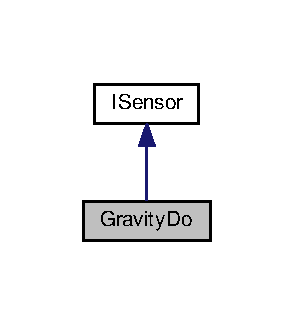
\includegraphics[width=141pt]{class_gravity_do__inherit__graph}
\end{center}
\end{figure}


Collaboration diagram for Gravity\+Do\+:\nopagebreak
\begin{figure}[H]
\begin{center}
\leavevmode
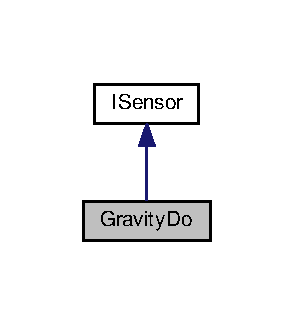
\includegraphics[width=141pt]{class_gravity_do__coll__graph}
\end{center}
\end{figure}
\subsection*{Public Member Functions}
\begin{DoxyCompactItemize}
\item 
void \hyperlink{class_gravity_do_a50230d3b101165f876cd595f5839e40b}{begin} ()
\item 
void \hyperlink{class_gravity_do_aafb8fcc3cdf0aac907288a0e5eb62b29}{update} ()
\item 
void {\bfseries set\+Pin} (int pin)\hypertarget{class_gravity_do_a6c4e78fad79943f86f4d5997307bd104}{}\label{class_gravity_do_a6c4e78fad79943f86f4d5997307bd104}

\item 
double \hyperlink{class_gravity_do_adaf18c91b1528ffbffceb097df12e54e}{get\+Value} ()
\item 
float {\bfseries get\+Temperature} () const \hypertarget{class_gravity_do_a116231bedc63f8ba338f798915b0fb94}{}\label{class_gravity_do_a116231bedc63f8ba338f798915b0fb94}

\item 
void {\bfseries set\+Temperature} (float temperature)\hypertarget{class_gravity_do_aa124f3b58a2315709b783dd64be1c276}{}\label{class_gravity_do_aa124f3b58a2315709b783dd64be1c276}

\end{DoxyCompactItemize}


\subsection{Member Function Documentation}
\index{Gravity\+Do@{Gravity\+Do}!begin@{begin}}
\index{begin@{begin}!Gravity\+Do@{Gravity\+Do}}
\subsubsection[{\texorpdfstring{begin()}{begin()}}]{\setlength{\rightskip}{0pt plus 5cm}void Gravity\+Do\+::begin (
\begin{DoxyParamCaption}
{}
\end{DoxyParamCaption}
)\hspace{0.3cm}{\ttfamily [virtual]}}\hypertarget{class_gravity_do_a50230d3b101165f876cd595f5839e40b}{}\label{class_gravity_do_a50230d3b101165f876cd595f5839e40b}
This function starts the sensor. All the initial configurations must be done here 

Implements \hyperlink{class_i_sensor_a88d0363e9bb83378090a021d634e03f7}{I\+Sensor}.

\index{Gravity\+Do@{Gravity\+Do}!get\+Value@{get\+Value}}
\index{get\+Value@{get\+Value}!Gravity\+Do@{Gravity\+Do}}
\subsubsection[{\texorpdfstring{get\+Value()}{getValue()}}]{\setlength{\rightskip}{0pt plus 5cm}double Gravity\+Do\+::get\+Value (
\begin{DoxyParamCaption}
{}
\end{DoxyParamCaption}
)\hspace{0.3cm}{\ttfamily [virtual]}}\hypertarget{class_gravity_do_adaf18c91b1528ffbffceb097df12e54e}{}\label{class_gravity_do_adaf18c91b1528ffbffceb097df12e54e}
This function must return the sensor data. You should run \hyperlink{class_gravity_do_aafb8fcc3cdf0aac907288a0e5eb62b29}{update()} just before \hyperlink{class_gravity_do_adaf18c91b1528ffbffceb097df12e54e}{get\+Value()} to return a recent and valid data. 

Implements \hyperlink{class_i_sensor_a9972b325fb329e6eaefd79e562ad7776}{I\+Sensor}.

\index{Gravity\+Do@{Gravity\+Do}!update@{update}}
\index{update@{update}!Gravity\+Do@{Gravity\+Do}}
\subsubsection[{\texorpdfstring{update()}{update()}}]{\setlength{\rightskip}{0pt plus 5cm}void Gravity\+Do\+::update (
\begin{DoxyParamCaption}
{}
\end{DoxyParamCaption}
)\hspace{0.3cm}{\ttfamily [virtual]}}\hypertarget{class_gravity_do_aafb8fcc3cdf0aac907288a0e5eb62b29}{}\label{class_gravity_do_aafb8fcc3cdf0aac907288a0e5eb62b29}
This function updates the sensor value and stores the value, so that it\textquotesingle{}s ready to return data 

Implements \hyperlink{class_i_sensor_a53606e8b3764eda1b4b0c00aa983e264}{I\+Sensor}.


\hypertarget{class_gravity_ec}{}\section{Gravity\+Ec Class Reference}
\label{class_gravity_ec}\index{Gravity\+Ec@{Gravity\+Ec}}


Inheritance diagram for Gravity\+Ec\+:\nopagebreak
\begin{figure}[H]
\begin{center}
\leavevmode
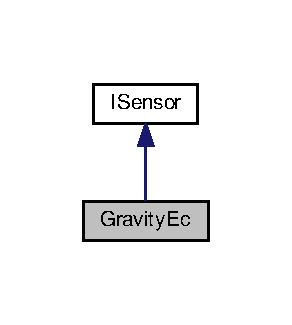
\includegraphics[width=140pt]{class_gravity_ec__inherit__graph}
\end{center}
\end{figure}


Collaboration diagram for Gravity\+Ec\+:\nopagebreak
\begin{figure}[H]
\begin{center}
\leavevmode
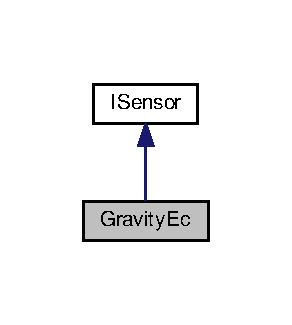
\includegraphics[width=140pt]{class_gravity_ec__coll__graph}
\end{center}
\end{figure}
\subsection*{Public Member Functions}
\begin{DoxyCompactItemize}
\item 
{\bfseries Gravity\+Ec} (\hyperlink{class_i_sensor}{I\+Sensor} $\ast$)\hypertarget{class_gravity_ec_a6907e34720f011cf7eed6a99c93ab66f}{}\label{class_gravity_ec_a6907e34720f011cf7eed6a99c93ab66f}

\item 
void {\bfseries begin} ()\hypertarget{class_gravity_ec_aab0f65470fdff7fb4465ecbbf57556a1}{}\label{class_gravity_ec_aab0f65470fdff7fb4465ecbbf57556a1}

\item 
void {\bfseries update} ()\hypertarget{class_gravity_ec_a8e0463b6147cfbcbc1488dd1614141c7}{}\label{class_gravity_ec_a8e0463b6147cfbcbc1488dd1614141c7}

\item 
double {\bfseries get\+Value} ()\hypertarget{class_gravity_ec_ac7307196ab402c5a65cbc8beb9dd7399}{}\label{class_gravity_ec_ac7307196ab402c5a65cbc8beb9dd7399}

\end{DoxyCompactItemize}
\subsection*{Public Attributes}
\begin{DoxyCompactItemize}
\item 
int {\bfseries ec\+Sensor\+Pin}\hypertarget{class_gravity_ec_a79c99fcfced63d1e170a5ed3fbf0146e}{}\label{class_gravity_ec_a79c99fcfced63d1e170a5ed3fbf0146e}

\item 
double {\bfseries E\+Ccurrent}\hypertarget{class_gravity_ec_a55b65815e70813e52e8dd66fc6db147b}{}\label{class_gravity_ec_a55b65815e70813e52e8dd66fc6db147b}

\end{DoxyCompactItemize}


The documentation for this class was generated from the following files\+:\begin{DoxyCompactItemize}
\item 
/home/henrique/arduino-\/1.\+8.\+9/libraries/\+Know\+Flow/Gravity\+Ec.\+h\item 
/home/henrique/arduino-\/1.\+8.\+9/libraries/\+Know\+Flow/Gravity\+Ec.\+cpp\end{DoxyCompactItemize}

\hypertarget{class_gravity_orp}{}\section{Gravity\+Orp Class Reference}
\label{class_gravity_orp}\index{Gravity\+Orp@{Gravity\+Orp}}


Inheritance diagram for Gravity\+Orp\+:\nopagebreak
\begin{figure}[H]
\begin{center}
\leavevmode
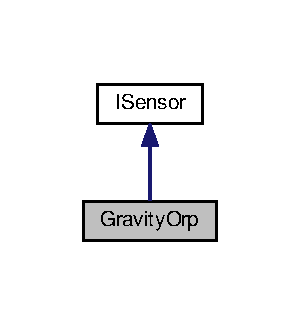
\includegraphics[width=144pt]{class_gravity_orp__inherit__graph}
\end{center}
\end{figure}


Collaboration diagram for Gravity\+Orp\+:\nopagebreak
\begin{figure}[H]
\begin{center}
\leavevmode
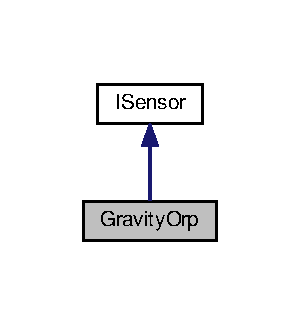
\includegraphics[width=144pt]{class_gravity_orp__coll__graph}
\end{center}
\end{figure}
\subsection*{Public Member Functions}
\begin{DoxyCompactItemize}
\item 
void \hyperlink{class_gravity_orp_a03543b2abbe0be53f2dfb799b22b3aef}{begin} ()
\item 
void \hyperlink{class_gravity_orp_aa39d1bf33bcf7f4f415fd51d8129d15a}{update} ()
\item 
double \hyperlink{class_gravity_orp_a2b4da109c95a3415fc70b9523bd13700}{get\+Value} ()
\end{DoxyCompactItemize}
\subsection*{Public Attributes}
\begin{DoxyCompactItemize}
\item 
int {\bfseries orp\+Sensor\+Pin}\hypertarget{class_gravity_orp_a3c70709c954fdba46ff218ed9084d16f}{}\label{class_gravity_orp_a3c70709c954fdba46ff218ed9084d16f}

\item 
double {\bfseries voltage}\hypertarget{class_gravity_orp_a0d0b0f34cb37014fd144a800388a17af}{}\label{class_gravity_orp_a0d0b0f34cb37014fd144a800388a17af}

\item 
float {\bfseries offset}\hypertarget{class_gravity_orp_a298092950afeb11b7c9e742887cb4b1f}{}\label{class_gravity_orp_a298092950afeb11b7c9e742887cb4b1f}

\end{DoxyCompactItemize}


\subsection{Member Function Documentation}
\index{Gravity\+Orp@{Gravity\+Orp}!begin@{begin}}
\index{begin@{begin}!Gravity\+Orp@{Gravity\+Orp}}
\subsubsection[{\texorpdfstring{begin()}{begin()}}]{\setlength{\rightskip}{0pt plus 5cm}void Gravity\+Orp\+::begin (
\begin{DoxyParamCaption}
{}
\end{DoxyParamCaption}
)\hspace{0.3cm}{\ttfamily [virtual]}}\hypertarget{class_gravity_orp_a03543b2abbe0be53f2dfb799b22b3aef}{}\label{class_gravity_orp_a03543b2abbe0be53f2dfb799b22b3aef}
This function starts the sensor. All the initial configurations must be done here 

Implements \hyperlink{class_i_sensor_a88d0363e9bb83378090a021d634e03f7}{I\+Sensor}.

\index{Gravity\+Orp@{Gravity\+Orp}!get\+Value@{get\+Value}}
\index{get\+Value@{get\+Value}!Gravity\+Orp@{Gravity\+Orp}}
\subsubsection[{\texorpdfstring{get\+Value()}{getValue()}}]{\setlength{\rightskip}{0pt plus 5cm}double Gravity\+Orp\+::get\+Value (
\begin{DoxyParamCaption}
{}
\end{DoxyParamCaption}
)\hspace{0.3cm}{\ttfamily [virtual]}}\hypertarget{class_gravity_orp_a2b4da109c95a3415fc70b9523bd13700}{}\label{class_gravity_orp_a2b4da109c95a3415fc70b9523bd13700}
This function must return the sensor data. You should run \hyperlink{class_gravity_orp_aa39d1bf33bcf7f4f415fd51d8129d15a}{update()} just before \hyperlink{class_gravity_orp_a2b4da109c95a3415fc70b9523bd13700}{get\+Value()} to return a recent and valid data. 

Implements \hyperlink{class_i_sensor_a9972b325fb329e6eaefd79e562ad7776}{I\+Sensor}.

\index{Gravity\+Orp@{Gravity\+Orp}!update@{update}}
\index{update@{update}!Gravity\+Orp@{Gravity\+Orp}}
\subsubsection[{\texorpdfstring{update()}{update()}}]{\setlength{\rightskip}{0pt plus 5cm}void Gravity\+Orp\+::update (
\begin{DoxyParamCaption}
{}
\end{DoxyParamCaption}
)\hspace{0.3cm}{\ttfamily [virtual]}}\hypertarget{class_gravity_orp_aa39d1bf33bcf7f4f415fd51d8129d15a}{}\label{class_gravity_orp_aa39d1bf33bcf7f4f415fd51d8129d15a}
This function updates the sensor value and stores the value, so that it\textquotesingle{}s ready to return data 

Implements \hyperlink{class_i_sensor_a53606e8b3764eda1b4b0c00aa983e264}{I\+Sensor}.


\hypertarget{class_gravity_ph}{}\section{Gravity\+Ph Class Reference}
\label{class_gravity_ph}\index{Gravity\+Ph@{Gravity\+Ph}}


Inheritance diagram for Gravity\+Ph\+:\nopagebreak
\begin{figure}[H]
\begin{center}
\leavevmode
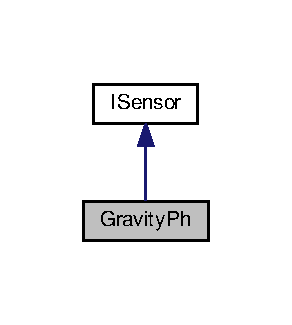
\includegraphics[width=140pt]{class_gravity_ph__inherit__graph}
\end{center}
\end{figure}


Collaboration diagram for Gravity\+Ph\+:\nopagebreak
\begin{figure}[H]
\begin{center}
\leavevmode
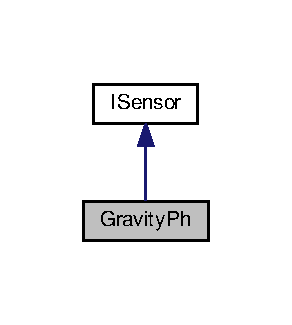
\includegraphics[width=140pt]{class_gravity_ph__coll__graph}
\end{center}
\end{figure}
\subsection*{Public Member Functions}
\begin{DoxyCompactItemize}
\item 
void \hyperlink{class_gravity_ph_a15c06b3c63d098a3b413e5cc97beb547}{begin} ()
\item 
void \hyperlink{class_gravity_ph_a3661f2d7ae52fcdcc7cde674e9a1e213}{update} ()
\item 
double \hyperlink{class_gravity_ph_a12f9ad86776c01409e0e3d4e3ab46178}{get\+Value} ()
\end{DoxyCompactItemize}
\subsection*{Public Attributes}
\begin{DoxyCompactItemize}
\item 
int {\bfseries ph\+Sensor\+Pin}\hypertarget{class_gravity_ph_a30ac3cfec7506aef36cca0ed94309171}{}\label{class_gravity_ph_a30ac3cfec7506aef36cca0ed94309171}

\item 
int {\bfseries sampling\+Interval}\hypertarget{class_gravity_ph_a2f0ead9fbd3614ea4e84223e2b26dd0e}{}\label{class_gravity_ph_a2f0ead9fbd3614ea4e84223e2b26dd0e}

\end{DoxyCompactItemize}


\subsection{Member Function Documentation}
\index{Gravity\+Ph@{Gravity\+Ph}!begin@{begin}}
\index{begin@{begin}!Gravity\+Ph@{Gravity\+Ph}}
\subsubsection[{\texorpdfstring{begin()}{begin()}}]{\setlength{\rightskip}{0pt plus 5cm}void Gravity\+Ph\+::begin (
\begin{DoxyParamCaption}
{}
\end{DoxyParamCaption}
)\hspace{0.3cm}{\ttfamily [virtual]}}\hypertarget{class_gravity_ph_a15c06b3c63d098a3b413e5cc97beb547}{}\label{class_gravity_ph_a15c06b3c63d098a3b413e5cc97beb547}
This function starts the sensor. All the initial configurations must be done here 

Implements \hyperlink{class_i_sensor_a88d0363e9bb83378090a021d634e03f7}{I\+Sensor}.

\index{Gravity\+Ph@{Gravity\+Ph}!get\+Value@{get\+Value}}
\index{get\+Value@{get\+Value}!Gravity\+Ph@{Gravity\+Ph}}
\subsubsection[{\texorpdfstring{get\+Value()}{getValue()}}]{\setlength{\rightskip}{0pt plus 5cm}double Gravity\+Ph\+::get\+Value (
\begin{DoxyParamCaption}
{}
\end{DoxyParamCaption}
)\hspace{0.3cm}{\ttfamily [virtual]}}\hypertarget{class_gravity_ph_a12f9ad86776c01409e0e3d4e3ab46178}{}\label{class_gravity_ph_a12f9ad86776c01409e0e3d4e3ab46178}
This function must return the sensor data. You should run \hyperlink{class_gravity_ph_a3661f2d7ae52fcdcc7cde674e9a1e213}{update()} just before \hyperlink{class_gravity_ph_a12f9ad86776c01409e0e3d4e3ab46178}{get\+Value()} to return a recent and valid data. 

Implements \hyperlink{class_i_sensor_a9972b325fb329e6eaefd79e562ad7776}{I\+Sensor}.

\index{Gravity\+Ph@{Gravity\+Ph}!update@{update}}
\index{update@{update}!Gravity\+Ph@{Gravity\+Ph}}
\subsubsection[{\texorpdfstring{update()}{update()}}]{\setlength{\rightskip}{0pt plus 5cm}void Gravity\+Ph\+::update (
\begin{DoxyParamCaption}
{}
\end{DoxyParamCaption}
)\hspace{0.3cm}{\ttfamily [virtual]}}\hypertarget{class_gravity_ph_a3661f2d7ae52fcdcc7cde674e9a1e213}{}\label{class_gravity_ph_a3661f2d7ae52fcdcc7cde674e9a1e213}
This function updates the sensor value and stores the value, so that it\textquotesingle{}s ready to return data 

Implements \hyperlink{class_i_sensor_a53606e8b3764eda1b4b0c00aa983e264}{I\+Sensor}.


\hypertarget{class_gravity_rtc}{}\section{Gravity\+Rtc Class Reference}
\label{class_gravity_rtc}\index{Gravity\+Rtc@{Gravity\+Rtc}}
\subsection*{Public Member Functions}
\begin{DoxyCompactItemize}
\item 
void {\bfseries adjust\+Rtc} (const \+\_\+\+\_\+\+Flash\+String\+Helper $\ast$date, const \+\_\+\+\_\+\+Flash\+String\+Helper $\ast$time)\hypertarget{class_gravity_rtc_af98ba41a948771253e5e936063a817d3}{}\label{class_gravity_rtc_af98ba41a948771253e5e936063a817d3}

\item 
void {\bfseries adjust\+Rtc} (uint16\+\_\+t year, uint8\+\_\+t month, uint8\+\_\+t day, uint8\+\_\+t week, uint8\+\_\+t hour, uint8\+\_\+t minute, uint8\+\_\+t second)\hypertarget{class_gravity_rtc_afd60ca78ef607244348873630ccf9259}{}\label{class_gravity_rtc_afd60ca78ef607244348873630ccf9259}

\item 
void {\bfseries setup} ()\hypertarget{class_gravity_rtc_ac4035c99a3e51f7b643628ab885c176b}{}\label{class_gravity_rtc_ac4035c99a3e51f7b643628ab885c176b}

\item 
void {\bfseries read} ()\hypertarget{class_gravity_rtc_ab4d3d5800f67e1362502be92107cd8b9}{}\label{class_gravity_rtc_ab4d3d5800f67e1362502be92107cd8b9}

\item 
uint16\+\_\+t {\bfseries get\+Year} ()\hypertarget{class_gravity_rtc_a35c000ff428ac2c0b46d1b490532b29f}{}\label{class_gravity_rtc_a35c000ff428ac2c0b46d1b490532b29f}

\item 
uint8\+\_\+t {\bfseries get\+Month} ()\hypertarget{class_gravity_rtc_aaacf3ae5e3521206560f3a23b64030cd}{}\label{class_gravity_rtc_aaacf3ae5e3521206560f3a23b64030cd}

\item 
uint8\+\_\+t {\bfseries get\+Day} ()\hypertarget{class_gravity_rtc_adb6f74357a48f49ac0596aac3f558c7d}{}\label{class_gravity_rtc_adb6f74357a48f49ac0596aac3f558c7d}

\item 
uint8\+\_\+t {\bfseries get\+Week} ()\hypertarget{class_gravity_rtc_aa3d944f570e2906faad6ab4b1aa35372}{}\label{class_gravity_rtc_aa3d944f570e2906faad6ab4b1aa35372}

\item 
uint8\+\_\+t {\bfseries get\+Hour} ()\hypertarget{class_gravity_rtc_adae161e4945aacae87a82f7d03b33f3a}{}\label{class_gravity_rtc_adae161e4945aacae87a82f7d03b33f3a}

\item 
uint8\+\_\+t {\bfseries get\+Minute} ()\hypertarget{class_gravity_rtc_a42038ee8675d49eae74ce75ee8bd4fa9}{}\label{class_gravity_rtc_a42038ee8675d49eae74ce75ee8bd4fa9}

\item 
uint8\+\_\+t {\bfseries get\+Second} ()\hypertarget{class_gravity_rtc_afb1a44b11e84bec28ed72e1b73068e54}{}\label{class_gravity_rtc_afb1a44b11e84bec28ed72e1b73068e54}

\end{DoxyCompactItemize}

\hypertarget{class_gravity_sensor_hub}{}\section{Gravity\+Sensor\+Hub Class Reference}
\label{class_gravity_sensor_hub}\index{Gravity\+Sensor\+Hub@{Gravity\+Sensor\+Hub}}


Collaboration diagram for Gravity\+Sensor\+Hub\+:\nopagebreak
\begin{figure}[H]
\begin{center}
\leavevmode
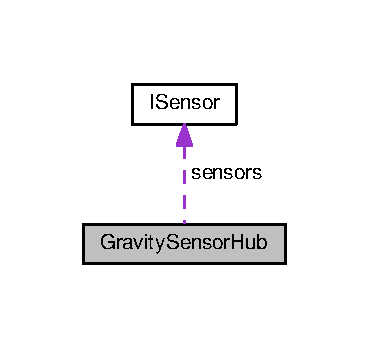
\includegraphics[width=177pt]{class_gravity_sensor_hub__coll__graph}
\end{center}
\end{figure}
\subsection*{Public Member Functions}
\begin{DoxyCompactItemize}
\item 
void {\bfseries begin} ()\hypertarget{class_gravity_sensor_hub_ad6e158e956ebaea865c5508b2f0fbacc}{}\label{class_gravity_sensor_hub_ad6e158e956ebaea865c5508b2f0fbacc}

\item 
void {\bfseries update} ()\hypertarget{class_gravity_sensor_hub_a5b253e5452c4860926b694922fc987f7}{}\label{class_gravity_sensor_hub_a5b253e5452c4860926b694922fc987f7}

\item 
double {\bfseries get\+Value\+By\+Sensor\+Number} (int num)\hypertarget{class_gravity_sensor_hub_a12fdc4fb6e3ec36d16fd92ae448ccc5d}{}\label{class_gravity_sensor_hub_a12fdc4fb6e3ec36d16fd92ae448ccc5d}

\end{DoxyCompactItemize}
\subsection*{Public Attributes}
\begin{DoxyCompactItemize}
\item 
\hyperlink{class_i_sensor}{I\+Sensor} $\ast$ {\bfseries sensors} \mbox{[}Sensor\+Count\mbox{]} = \{0\}\hypertarget{class_gravity_sensor_hub_ae7bd459a1ca0eb6b2ac748f7c288a7d0}{}\label{class_gravity_sensor_hub_ae7bd459a1ca0eb6b2ac748f7c288a7d0}

\end{DoxyCompactItemize}


The documentation for this class was generated from the following files\+:\begin{DoxyCompactItemize}
\item 
/home/henrique/arduino-\/1.\+8.\+9/libraries/\+Know\+Flow/Gravity\+Sensor\+Hub.\+h\item 
/home/henrique/arduino-\/1.\+8.\+9/libraries/\+Know\+Flow/Gravity\+Sensor\+Hub.\+cpp\end{DoxyCompactItemize}

\hypertarget{class_gravity_t_d_s}{}\section{Gravity\+T\+DS Class Reference}
\label{class_gravity_t_d_s}\index{Gravity\+T\+DS@{Gravity\+T\+DS}}


Inheritance diagram for Gravity\+T\+DS\+:\nopagebreak
\begin{figure}[H]
\begin{center}
\leavevmode
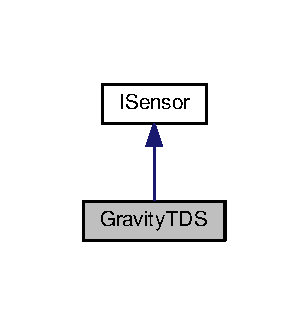
\includegraphics[width=148pt]{class_gravity_t_d_s__inherit__graph}
\end{center}
\end{figure}


Collaboration diagram for Gravity\+T\+DS\+:\nopagebreak
\begin{figure}[H]
\begin{center}
\leavevmode
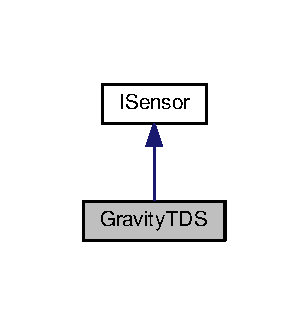
\includegraphics[width=148pt]{class_gravity_t_d_s__coll__graph}
\end{center}
\end{figure}
\subsection*{Public Member Functions}
\begin{DoxyCompactItemize}
\item 
void {\bfseries begin} ()\hypertarget{class_gravity_t_d_s_a1918273706ab9bfafe2e9a3ea3a61171}{}\label{class_gravity_t_d_s_a1918273706ab9bfafe2e9a3ea3a61171}

\item 
void {\bfseries update} ()\hypertarget{class_gravity_t_d_s_a56be401a2aa89a4918319e0d8262ea48}{}\label{class_gravity_t_d_s_a56be401a2aa89a4918319e0d8262ea48}

\item 
double {\bfseries get\+Value} ()\hypertarget{class_gravity_t_d_s_a9812b355ecc031f1dfb7039208f1c170}{}\label{class_gravity_t_d_s_a9812b355ecc031f1dfb7039208f1c170}

\item 
void {\bfseries set\+Pin} (int pin)\hypertarget{class_gravity_t_d_s_a9a91e8461f6696ffff169c456eb9cbac}{}\label{class_gravity_t_d_s_a9a91e8461f6696ffff169c456eb9cbac}

\item 
float {\bfseries set\+Temperature} (float temp)\hypertarget{class_gravity_t_d_s_a000fe439b71ff425ddbb27d5bfd480a9}{}\label{class_gravity_t_d_s_a000fe439b71ff425ddbb27d5bfd480a9}

\item 
float {\bfseries set\+Vref} (float value)\hypertarget{class_gravity_t_d_s_ab7732b7a1ac0c4725b48d9c601830176}{}\label{class_gravity_t_d_s_ab7732b7a1ac0c4725b48d9c601830176}

\end{DoxyCompactItemize}


The documentation for this class was generated from the following files\+:\begin{DoxyCompactItemize}
\item 
/home/henrique/arduino-\/1.\+8.\+9/libraries/\+Know\+Flow/Gravity\+T\+D\+S.\+h\item 
/home/henrique/arduino-\/1.\+8.\+9/libraries/\+Know\+Flow/Gravity\+T\+D\+S.\+cpp\end{DoxyCompactItemize}

\hypertarget{class_gravity_temperature}{}\section{Gravity\+Temperature Class Reference}
\label{class_gravity_temperature}\index{Gravity\+Temperature@{Gravity\+Temperature}}


Inheritance diagram for Gravity\+Temperature\+:\nopagebreak
\begin{figure}[H]
\begin{center}
\leavevmode
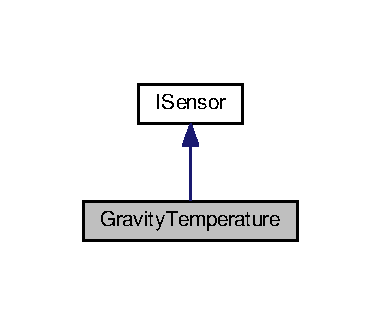
\includegraphics[width=183pt]{class_gravity_temperature__inherit__graph}
\end{center}
\end{figure}


Collaboration diagram for Gravity\+Temperature\+:\nopagebreak
\begin{figure}[H]
\begin{center}
\leavevmode
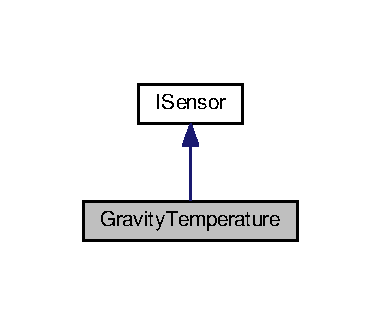
\includegraphics[width=183pt]{class_gravity_temperature__coll__graph}
\end{center}
\end{figure}
\subsection*{Public Member Functions}
\begin{DoxyCompactItemize}
\item 
{\bfseries Gravity\+Temperature} (int pin)\hypertarget{class_gravity_temperature_a1156c03146096ebd11dfeb12d047b017}{}\label{class_gravity_temperature_a1156c03146096ebd11dfeb12d047b017}

\item 
void \hyperlink{class_gravity_temperature_a4b0e6bba015c69a153a85cc8221dee2f}{begin} ()
\item 
void \hyperlink{class_gravity_temperature_aa7a3463559fe46fa4471f779fb5ffdce}{update} ()
\item 
double \hyperlink{class_gravity_temperature_a7ee39e7ab5521f9dcbdea543c26c3a26}{get\+Value} ()
\end{DoxyCompactItemize}
\subsection*{Public Attributes}
\begin{DoxyCompactItemize}
\item 
int {\bfseries temperature\+Pin}\hypertarget{class_gravity_temperature_a12137835ad1ee47f2e5d940d74c02628}{}\label{class_gravity_temperature_a12137835ad1ee47f2e5d940d74c02628}

\item 
double {\bfseries temperature}\hypertarget{class_gravity_temperature_a6a4ea3f7581c3d3f18269492c7cc5c85}{}\label{class_gravity_temperature_a6a4ea3f7581c3d3f18269492c7cc5c85}

\end{DoxyCompactItemize}


\subsection{Member Function Documentation}
\index{Gravity\+Temperature@{Gravity\+Temperature}!begin@{begin}}
\index{begin@{begin}!Gravity\+Temperature@{Gravity\+Temperature}}
\subsubsection[{\texorpdfstring{begin()}{begin()}}]{\setlength{\rightskip}{0pt plus 5cm}void Gravity\+Temperature\+::begin (
\begin{DoxyParamCaption}
{}
\end{DoxyParamCaption}
)\hspace{0.3cm}{\ttfamily [virtual]}}\hypertarget{class_gravity_temperature_a4b0e6bba015c69a153a85cc8221dee2f}{}\label{class_gravity_temperature_a4b0e6bba015c69a153a85cc8221dee2f}
This function starts the sensor. All the initial configurations must be done here 

Implements \hyperlink{class_i_sensor_a88d0363e9bb83378090a021d634e03f7}{I\+Sensor}.

\index{Gravity\+Temperature@{Gravity\+Temperature}!get\+Value@{get\+Value}}
\index{get\+Value@{get\+Value}!Gravity\+Temperature@{Gravity\+Temperature}}
\subsubsection[{\texorpdfstring{get\+Value()}{getValue()}}]{\setlength{\rightskip}{0pt plus 5cm}double Gravity\+Temperature\+::get\+Value (
\begin{DoxyParamCaption}
{}
\end{DoxyParamCaption}
)\hspace{0.3cm}{\ttfamily [virtual]}}\hypertarget{class_gravity_temperature_a7ee39e7ab5521f9dcbdea543c26c3a26}{}\label{class_gravity_temperature_a7ee39e7ab5521f9dcbdea543c26c3a26}
This function must return the sensor data. You should run \hyperlink{class_gravity_temperature_aa7a3463559fe46fa4471f779fb5ffdce}{update()} just before \hyperlink{class_gravity_temperature_a7ee39e7ab5521f9dcbdea543c26c3a26}{get\+Value()} to return a recent and valid data. 

Implements \hyperlink{class_i_sensor_a9972b325fb329e6eaefd79e562ad7776}{I\+Sensor}.

\index{Gravity\+Temperature@{Gravity\+Temperature}!update@{update}}
\index{update@{update}!Gravity\+Temperature@{Gravity\+Temperature}}
\subsubsection[{\texorpdfstring{update()}{update()}}]{\setlength{\rightskip}{0pt plus 5cm}void Gravity\+Temperature\+::update (
\begin{DoxyParamCaption}
{}
\end{DoxyParamCaption}
)\hspace{0.3cm}{\ttfamily [virtual]}}\hypertarget{class_gravity_temperature_aa7a3463559fe46fa4471f779fb5ffdce}{}\label{class_gravity_temperature_aa7a3463559fe46fa4471f779fb5ffdce}
This function updates the sensor value and stores the value, so that it\textquotesingle{}s ready to return data 

Implements \hyperlink{class_i_sensor_a53606e8b3764eda1b4b0c00aa983e264}{I\+Sensor}.


\hypertarget{class_i_sensor}{}\section{I\+Sensor Class Reference}
\label{class_i_sensor}\index{I\+Sensor@{I\+Sensor}}


Inheritance diagram for I\+Sensor\+:\nopagebreak
\begin{figure}[H]
\begin{center}
\leavevmode
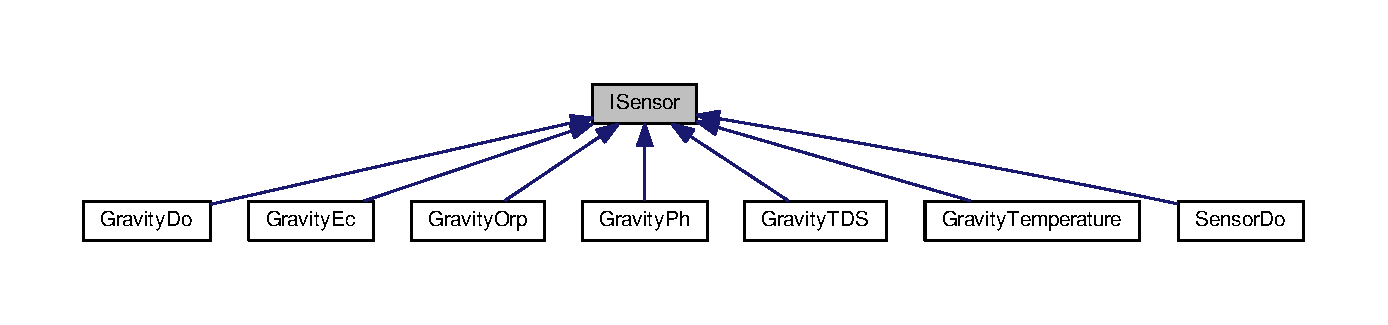
\includegraphics[width=350pt]{class_i_sensor__inherit__graph}
\end{center}
\end{figure}
\subsection*{Public Member Functions}
\begin{DoxyCompactItemize}
\item 
virtual void {\bfseries begin} ()=0\hypertarget{class_i_sensor_a88d0363e9bb83378090a021d634e03f7}{}\label{class_i_sensor_a88d0363e9bb83378090a021d634e03f7}

\item 
virtual void {\bfseries update} ()=0\hypertarget{class_i_sensor_a53606e8b3764eda1b4b0c00aa983e264}{}\label{class_i_sensor_a53606e8b3764eda1b4b0c00aa983e264}

\item 
virtual double {\bfseries get\+Value} ()=0\hypertarget{class_i_sensor_a9972b325fb329e6eaefd79e562ad7776}{}\label{class_i_sensor_a9972b325fb329e6eaefd79e562ad7776}

\end{DoxyCompactItemize}


The documentation for this class was generated from the following file\+:\begin{DoxyCompactItemize}
\item 
/home/henrique/arduino-\/1.\+8.\+9/libraries/\+Know\+Flow/I\+Sensor.\+h\end{DoxyCompactItemize}

\hypertarget{class_sd_service}{}\section{Sd\+Service Class Reference}
\label{class_sd_service}\index{Sd\+Service@{Sd\+Service}}
\subsection*{Public Member Functions}
\begin{DoxyCompactItemize}
\item 
{\bfseries Sd\+Service} (\hyperlink{class_i_sensor}{I\+Sensor} $\ast$gravity\+Sensor\mbox{[}$\,$\mbox{]})\hypertarget{class_sd_service_afed7960e6a28c171ffe552c88cfe4624}{}\label{class_sd_service_afed7960e6a28c171ffe552c88cfe4624}

\item 
void {\bfseries begin} ()\hypertarget{class_sd_service_a5c6e09a57f22f163676a51eab6f933c5}{}\label{class_sd_service_a5c6e09a57f22f163676a51eab6f933c5}

\item 
void {\bfseries update} ()\hypertarget{class_sd_service_a776b1a8d229b9b0bc44cbf6ae9b37c9d}{}\label{class_sd_service_a776b1a8d229b9b0bc44cbf6ae9b37c9d}

\end{DoxyCompactItemize}
\subsection*{Public Attributes}
\begin{DoxyCompactItemize}
\item 
int {\bfseries chip\+Select}\hypertarget{class_sd_service_a173f33cc9797e3ce4e213a75e627d2c9}{}\label{class_sd_service_a173f33cc9797e3ce4e213a75e627d2c9}

\end{DoxyCompactItemize}

\hypertarget{class_sensor_do}{}\section{Sensor\+Do Class Reference}
\label{class_sensor_do}\index{Sensor\+Do@{Sensor\+Do}}


{\ttfamily \#include $<$Sensor\+Do.\+h$>$}



Inheritance diagram for Sensor\+Do\+:\nopagebreak
\begin{figure}[H]
\begin{center}
\leavevmode
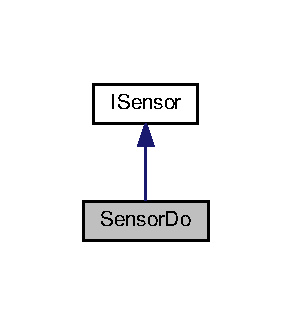
\includegraphics[width=140pt]{class_sensor_do__inherit__graph}
\end{center}
\end{figure}


Collaboration diagram for Sensor\+Do\+:\nopagebreak
\begin{figure}[H]
\begin{center}
\leavevmode
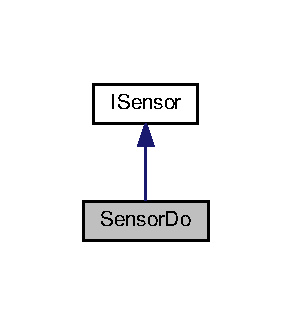
\includegraphics[width=140pt]{class_sensor_do__coll__graph}
\end{center}
\end{figure}
\subsection*{Public Member Functions}
\begin{DoxyCompactItemize}
\item 
\hyperlink{class_sensor_do_a04dabd201f2ceea94caea74533893790}{Sensor\+Do} ()
\item 
\hyperlink{class_sensor_do_a79740d3a503eb4668805572fa03962cd}{Sensor\+Do} (Stream \&st)
\item 
void \hyperlink{class_sensor_do_a211a11e96355ab492b1fa4b45a9d9f8c}{begin} ()
\item 
void \hyperlink{class_sensor_do_ab3a8e46368a78e5252e10ffd57caa6ee}{begin} (Stream \&st)
\item 
void \hyperlink{class_sensor_do_ae0d28d943e612b1a840a0b5e5bd5566d}{update} ()
\item 
double \hyperlink{class_sensor_do_a811d2c2e9dac3246763889226955a064}{get\+Value} ()
\end{DoxyCompactItemize}


\subsection{Detailed Description}
This class controls the \href{https://www.atlas-scientific.com/product_pages/kits/do_kit.html}{\tt Atlas Scientific DO Sensor} via uart serial interface. It takes Dissolved Oxigen readings from the \href{https://www.atlas-scientific.com/_files/_datasheets/_circuit/DO_EZO_Datasheet.pdf?}{\tt E\+ZO} circuit and stores it\textquotesingle{}s current value. 

\subsection{Constructor \& Destructor Documentation}
\index{Sensor\+Do@{Sensor\+Do}!Sensor\+Do@{Sensor\+Do}}
\index{Sensor\+Do@{Sensor\+Do}!Sensor\+Do@{Sensor\+Do}}
\subsubsection[{\texorpdfstring{Sensor\+Do()}{SensorDo()}}]{\setlength{\rightskip}{0pt plus 5cm}Sensor\+Do\+::\+Sensor\+Do (
\begin{DoxyParamCaption}
{}
\end{DoxyParamCaption}
)}\hypertarget{class_sensor_do_a04dabd201f2ceea94caea74533893790}{}\label{class_sensor_do_a04dabd201f2ceea94caea74533893790}
Default constructor. Sets the instantiated Hardware\+Serial Serial as the Stream for the sensor. \index{Sensor\+Do@{Sensor\+Do}!Sensor\+Do@{Sensor\+Do}}
\index{Sensor\+Do@{Sensor\+Do}!Sensor\+Do@{Sensor\+Do}}
\subsubsection[{\texorpdfstring{Sensor\+Do(\+Stream \&st)}{SensorDo(Stream &st)}}]{\setlength{\rightskip}{0pt plus 5cm}Sensor\+Do\+::\+Sensor\+Do (
\begin{DoxyParamCaption}
\item[{Stream \&}]{st}
\end{DoxyParamCaption}
)}\hypertarget{class_sensor_do_a79740d3a503eb4668805572fa03962cd}{}\label{class_sensor_do_a79740d3a503eb4668805572fa03962cd}
Initialize the Do Sensor with a given Stream. 
\begin{DoxyParams}[1]{Parameters}
\mbox{\tt in}  & {\em st} & The Stream for comunicate with the sensor via serial interface. \\
\hline
\end{DoxyParams}


\subsection{Member Function Documentation}
\index{Sensor\+Do@{Sensor\+Do}!begin@{begin}}
\index{begin@{begin}!Sensor\+Do@{Sensor\+Do}}
\subsubsection[{\texorpdfstring{begin()}{begin()}}]{\setlength{\rightskip}{0pt plus 5cm}void Sensor\+Do\+::begin (
\begin{DoxyParamCaption}
{}
\end{DoxyParamCaption}
)\hspace{0.3cm}{\ttfamily [virtual]}}\hypertarget{class_sensor_do_a211a11e96355ab492b1fa4b45a9d9f8c}{}\label{class_sensor_do_a211a11e96355ab492b1fa4b45a9d9f8c}
Initializes the default Serial instance 

Implements \hyperlink{class_i_sensor_a88d0363e9bb83378090a021d634e03f7}{I\+Sensor}.

\index{Sensor\+Do@{Sensor\+Do}!begin@{begin}}
\index{begin@{begin}!Sensor\+Do@{Sensor\+Do}}
\subsubsection[{\texorpdfstring{begin(\+Stream \&st)}{begin(Stream &st)}}]{\setlength{\rightskip}{0pt plus 5cm}void Sensor\+Do\+::begin (
\begin{DoxyParamCaption}
\item[{Stream \&}]{st}
\end{DoxyParamCaption}
)}\hypertarget{class_sensor_do_ab3a8e46368a78e5252e10ffd57caa6ee}{}\label{class_sensor_do_ab3a8e46368a78e5252e10ffd57caa6ee}
Initializes the DO sensor with a given Stream 
\begin{DoxyParams}[1]{Parameters}
\mbox{\tt in}  & {\em st} & The Stream for comunicating with the sensor via serial interface. \\
\hline
\end{DoxyParams}
\index{Sensor\+Do@{Sensor\+Do}!get\+Value@{get\+Value}}
\index{get\+Value@{get\+Value}!Sensor\+Do@{Sensor\+Do}}
\subsubsection[{\texorpdfstring{get\+Value()}{getValue()}}]{\setlength{\rightskip}{0pt plus 5cm}double Sensor\+Do\+::get\+Value (
\begin{DoxyParamCaption}
{}
\end{DoxyParamCaption}
)\hspace{0.3cm}{\ttfamily [virtual]}}\hypertarget{class_sensor_do_a811d2c2e9dac3246763889226955a064}{}\label{class_sensor_do_a811d2c2e9dac3246763889226955a064}
Read the stored value. \begin{DoxyReturn}{Returns}
The value os the sensor. 
\end{DoxyReturn}


Implements \hyperlink{class_i_sensor_a9972b325fb329e6eaefd79e562ad7776}{I\+Sensor}.

\index{Sensor\+Do@{Sensor\+Do}!update@{update}}
\index{update@{update}!Sensor\+Do@{Sensor\+Do}}
\subsubsection[{\texorpdfstring{update()}{update()}}]{\setlength{\rightskip}{0pt plus 5cm}void Sensor\+Do\+::update (
\begin{DoxyParamCaption}
{}
\end{DoxyParamCaption}
)\hspace{0.3cm}{\ttfamily [virtual]}}\hypertarget{class_sensor_do_ae0d28d943e612b1a840a0b5e5bd5566d}{}\label{class_sensor_do_ae0d28d943e612b1a840a0b5e5bd5566d}
Reads the sensor value and stores it\textquotesingle{}s value. 

Implements \hyperlink{class_i_sensor_a53606e8b3764eda1b4b0c00aa983e264}{I\+Sensor}.


\hypertarget{class_sensor_log}{}\section{Sensor\+Log Class Reference}
\label{class_sensor_log}\index{Sensor\+Log@{Sensor\+Log}}
\subsection*{Public Member Functions}
\begin{DoxyCompactItemize}
\item 
void {\bfseries create\+File} (String file\+Name)\hypertarget{class_sensor_log_a2e3d6b7483e6f739cfecb89b04c5a034}{}\label{class_sensor_log_a2e3d6b7483e6f739cfecb89b04c5a034}

\item 
void {\bfseries store\+Line} ()\hypertarget{class_sensor_log_a099560f4b46211476b0d112e8322f890}{}\label{class_sensor_log_a099560f4b46211476b0d112e8322f890}

\end{DoxyCompactItemize}

\chapter{File Documentation}
\hypertarget{_config_8h}{}\section{/home/henrique/arduino-\/1.8.9/libraries/\+Know\+Flow/\+Config.h File Reference}
\label{_config_8h}\index{/home/henrique/arduino-\/1.\+8.\+9/libraries/\+Know\+Flow/\+Config.\+h@{/home/henrique/arduino-\/1.\+8.\+9/libraries/\+Know\+Flow/\+Config.\+h}}
This graph shows which files directly or indirectly include this file\+:\nopagebreak
\begin{figure}[H]
\begin{center}
\leavevmode
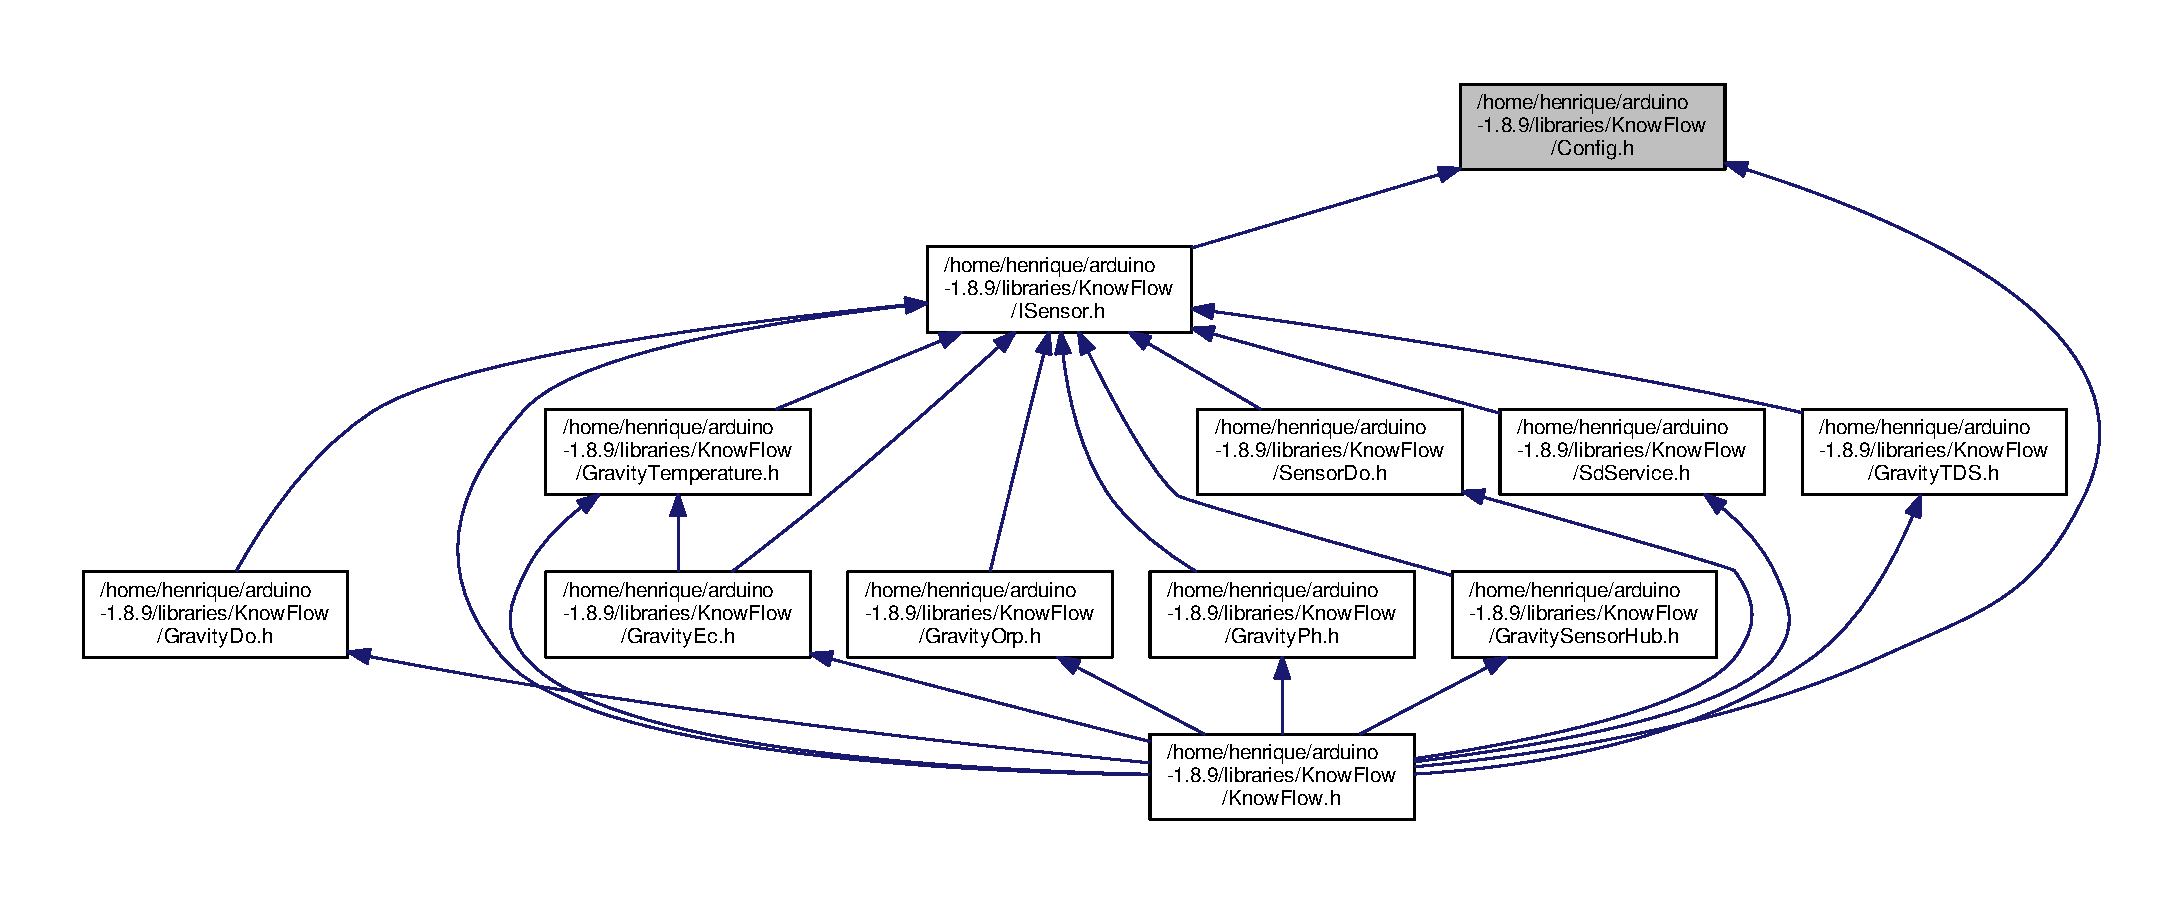
\includegraphics[width=350pt]{_config_8h__dep__incl}
\end{center}
\end{figure}
\subsection*{Macros}
\begin{DoxyCompactItemize}
\item 
\#define \hyperlink{_config_8h_a36f25ff2fdc455f9ae74e30b2713935e}{D\+E\+B\+U\+G\+\_\+\+A\+VR}
\item 
\#define \hyperlink{_config_8h_a47cea535cdbbf8046cf11fd1eee12fe5}{A\+R\+R\+A\+Y\+L\+E\+N\+G\+TH}~10\hypertarget{_config_8h_a47cea535cdbbf8046cf11fd1eee12fe5}{}\label{_config_8h_a47cea535cdbbf8046cf11fd1eee12fe5}

\begin{DoxyCompactList}\small\item\em The maximum length of the sensor filter array. \end{DoxyCompactList}\item 
\#define \hyperlink{_config_8h_a85c19c2498565182d196f9b145035fde}{S\+D\+U\+P\+D\+A\+T\+E\+D\+A\+T\+A\+T\+I\+ME}~60000\hypertarget{_config_8h_a85c19c2498565182d196f9b145035fde}{}\label{_config_8h_a85c19c2498565182d196f9b145035fde}

\begin{DoxyCompactList}\small\item\em SD card update data time, 60,000 is 1 minute. \end{DoxyCompactList}\item 
\#define \hyperlink{_config_8h_ad85919ae5261767d33875fe5cb0df6d8}{S\+E\+L\+E\+C\+T\+EC}\hypertarget{_config_8h_ad85919ae5261767d33875fe5cb0df6d8}{}\label{_config_8h_ad85919ae5261767d33875fe5cb0df6d8}

\begin{DoxyCompactList}\small\item\em EC sensor is selected by default, comment this line to use T\+DS sensor. \end{DoxyCompactList}\item 
\#define \hyperlink{group___p_i_n___s_e_t_t_i_n_g_s_gabaa87b795b67d2f09dcda7e30c939e2b}{D\+O\+P\+IN}~A0
\item 
\#define \hyperlink{group___p_i_n___s_e_t_t_i_n_g_s_ga9eea325c048cdcab4c3b5f9771f7b512}{E\+C\+P\+IN}~A1
\item 
\#define \hyperlink{group___p_i_n___s_e_t_t_i_n_g_s_gaef0cf2dcc531d0afe308cb1ed8ab951a}{T\+D\+S\+P\+IN}~A1
\item 
\#define \hyperlink{group___p_i_n___s_e_t_t_i_n_g_s_ga992fbb764f982b28e19730a8327b67a6}{P\+H\+P\+IN}~A2
\item 
\#define \hyperlink{group___p_i_n___s_e_t_t_i_n_g_s_ga2f2dcc0d9b12ba6a368d780187c98017}{O\+R\+P\+P\+IN}~A3
\item 
\#define \hyperlink{group___p_i_n___s_e_t_t_i_n_g_s_ga4ba38e7a40eda1fcddf502aa2265c313}{T\+E\+M\+P\+P\+IN}~5
\item 
\#define \hyperlink{_config_8h_a2a353ec5131082cab500ebbfd471615a}{P\+H\+O\+F\+F\+S\+ET}~0.\+12
\item 
\#define {\bfseries E\+C\+K\+V\+A\+L\+UE}~0.\+6\hypertarget{_config_8h_a5d6b9565a7ed78be7e49625169ba87e5}{}\label{_config_8h_a5d6b9565a7ed78be7e49625169ba87e5}

\item 
\#define \hyperlink{group___c_a_l___c_o_e_f_f_gabe5c1bc9018d7fb405b0f69c568d866b}{P\+H\+\_\+\+M\+\_\+\+C\+O\+E\+FF}~4.\+411
\item 
\#define \hyperlink{group___c_a_l___c_o_e_f_f_ga3d9cbf54f9b4b5ac4915d7d176e77bfe}{P\+H\+\_\+\+B\+\_\+\+C\+O\+E\+FF}~-\/0.\+014
\item 
\#define \hyperlink{group___c_a_l___c_o_e_f_f_gafd22da5c5584608227366042cdc86166}{O\+R\+P\+\_\+\+O\+F\+F\+S\+ET}~8.\+79
\item 
\#define \hyperlink{group___a_r_r_a_y___d_e_f_s_ga462faefe5424328c9f713503ecafeb6f}{S\+E\+N\+S\+O\+R\+C\+O\+U\+NT}~5
\item 
\#define \hyperlink{group___a_r_r_a_y___d_e_f_s_gaad8cbdb71736e79d15b2699c50b5dbfd}{P\+H\+\_\+\+I\+N\+D\+EX}~0
\item 
\#define \hyperlink{group___a_r_r_a_y___d_e_f_s_ga87282d20e6a935e76f14d903959695b5}{T\+E\+M\+P\+\_\+\+I\+N\+D\+EX}~1
\item 
\#define \hyperlink{group___a_r_r_a_y___d_e_f_s_gae984a0da3b36fc26bc8c5c79ac1fc1fa}{D\+O\+\_\+\+I\+N\+D\+EX}~2
\item 
\#define \hyperlink{group___a_r_r_a_y___d_e_f_s_ga01f1891f3723e0d0f6466d0afadf8e16}{E\+C\+\_\+\+I\+N\+D\+EX}~3
\item 
\#define \hyperlink{group___a_r_r_a_y___d_e_f_s_ga855d2056682afca7f6fab69afcc65b6a}{T\+D\+S\+\_\+\+I\+N\+D\+EX}~3
\item 
\#define \hyperlink{group___a_r_r_a_y___d_e_f_s_ga7104f69c9df0ea675fddbf7cf1b4ec22}{O\+R\+P\+\_\+\+I\+N\+D\+EX}~4
\end{DoxyCompactItemize}
\subsection*{Enumerations}
\begin{DoxyCompactItemize}
\item 
enum {\bfseries Sensor\+Number} \{ \\*
{\bfseries ph\+Sensor} = 0, 
{\bfseries temperature\+Sensor}, 
{\bfseries do\+Sensor}, 
{\bfseries ec\+Sensor}, 
\\*
{\bfseries tds\+Sensor} = 3, 
{\bfseries orp\+Sensor}
 \}\hypertarget{_config_8h_a524458713131934a168df3f7976140eb}{}\label{_config_8h_a524458713131934a168df3f7976140eb}

\end{DoxyCompactItemize}


\subsection{Macro Definition Documentation}
\index{Config.\+h@{Config.\+h}!D\+E\+B\+U\+G\+\_\+\+A\+VR@{D\+E\+B\+U\+G\+\_\+\+A\+VR}}
\index{D\+E\+B\+U\+G\+\_\+\+A\+VR@{D\+E\+B\+U\+G\+\_\+\+A\+VR}!Config.\+h@{Config.\+h}}
\subsubsection[{\texorpdfstring{D\+E\+B\+U\+G\+\_\+\+A\+VR}{DEBUG_AVR}}]{\setlength{\rightskip}{0pt plus 5cm}\#define D\+E\+B\+U\+G\+\_\+\+A\+VR}\hypertarget{_config_8h_a36f25ff2fdc455f9ae74e30b2713935e}{}\label{_config_8h_a36f25ff2fdc455f9ae74e30b2713935e}
Serial print switch \index{Config.\+h@{Config.\+h}!P\+H\+O\+F\+F\+S\+ET@{P\+H\+O\+F\+F\+S\+ET}}
\index{P\+H\+O\+F\+F\+S\+ET@{P\+H\+O\+F\+F\+S\+ET}!Config.\+h@{Config.\+h}}
\subsubsection[{\texorpdfstring{P\+H\+O\+F\+F\+S\+ET}{PHOFFSET}}]{\setlength{\rightskip}{0pt plus 5cm}\#define P\+H\+O\+F\+F\+S\+ET~0.\+12}\hypertarget{_config_8h_a2a353ec5131082cab500ebbfd471615a}{}\label{_config_8h_a2a353ec5131082cab500ebbfd471615a}
Set sensor offset (calibration data) 
\hypertarget{_i_sensor_8h}{}\section{/home/henrique/arduino-\/1.8.9/libraries/\+Know\+Flow/\+I\+Sensor.h File Reference}
\label{_i_sensor_8h}\index{/home/henrique/arduino-\/1.\+8.\+9/libraries/\+Know\+Flow/\+I\+Sensor.\+h@{/home/henrique/arduino-\/1.\+8.\+9/libraries/\+Know\+Flow/\+I\+Sensor.\+h}}


This class represents a generic sensor.  


{\ttfamily \#include \char`\"{}Config.\+h\char`\"{}}\\*
{\ttfamily \#include \char`\"{}Arduino.\+h\char`\"{}}\\*
Include dependency graph for I\+Sensor.\+h\+:\nopagebreak
\begin{figure}[H]
\begin{center}
\leavevmode
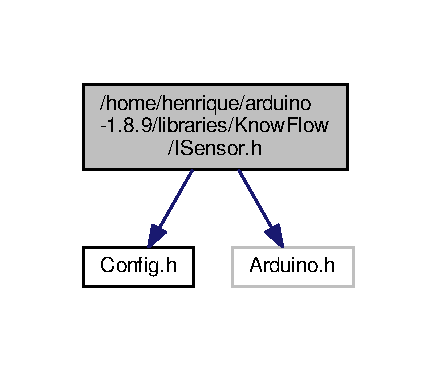
\includegraphics[width=210pt]{_i_sensor_8h__incl}
\end{center}
\end{figure}
This graph shows which files directly or indirectly include this file\+:
\nopagebreak
\begin{figure}[H]
\begin{center}
\leavevmode
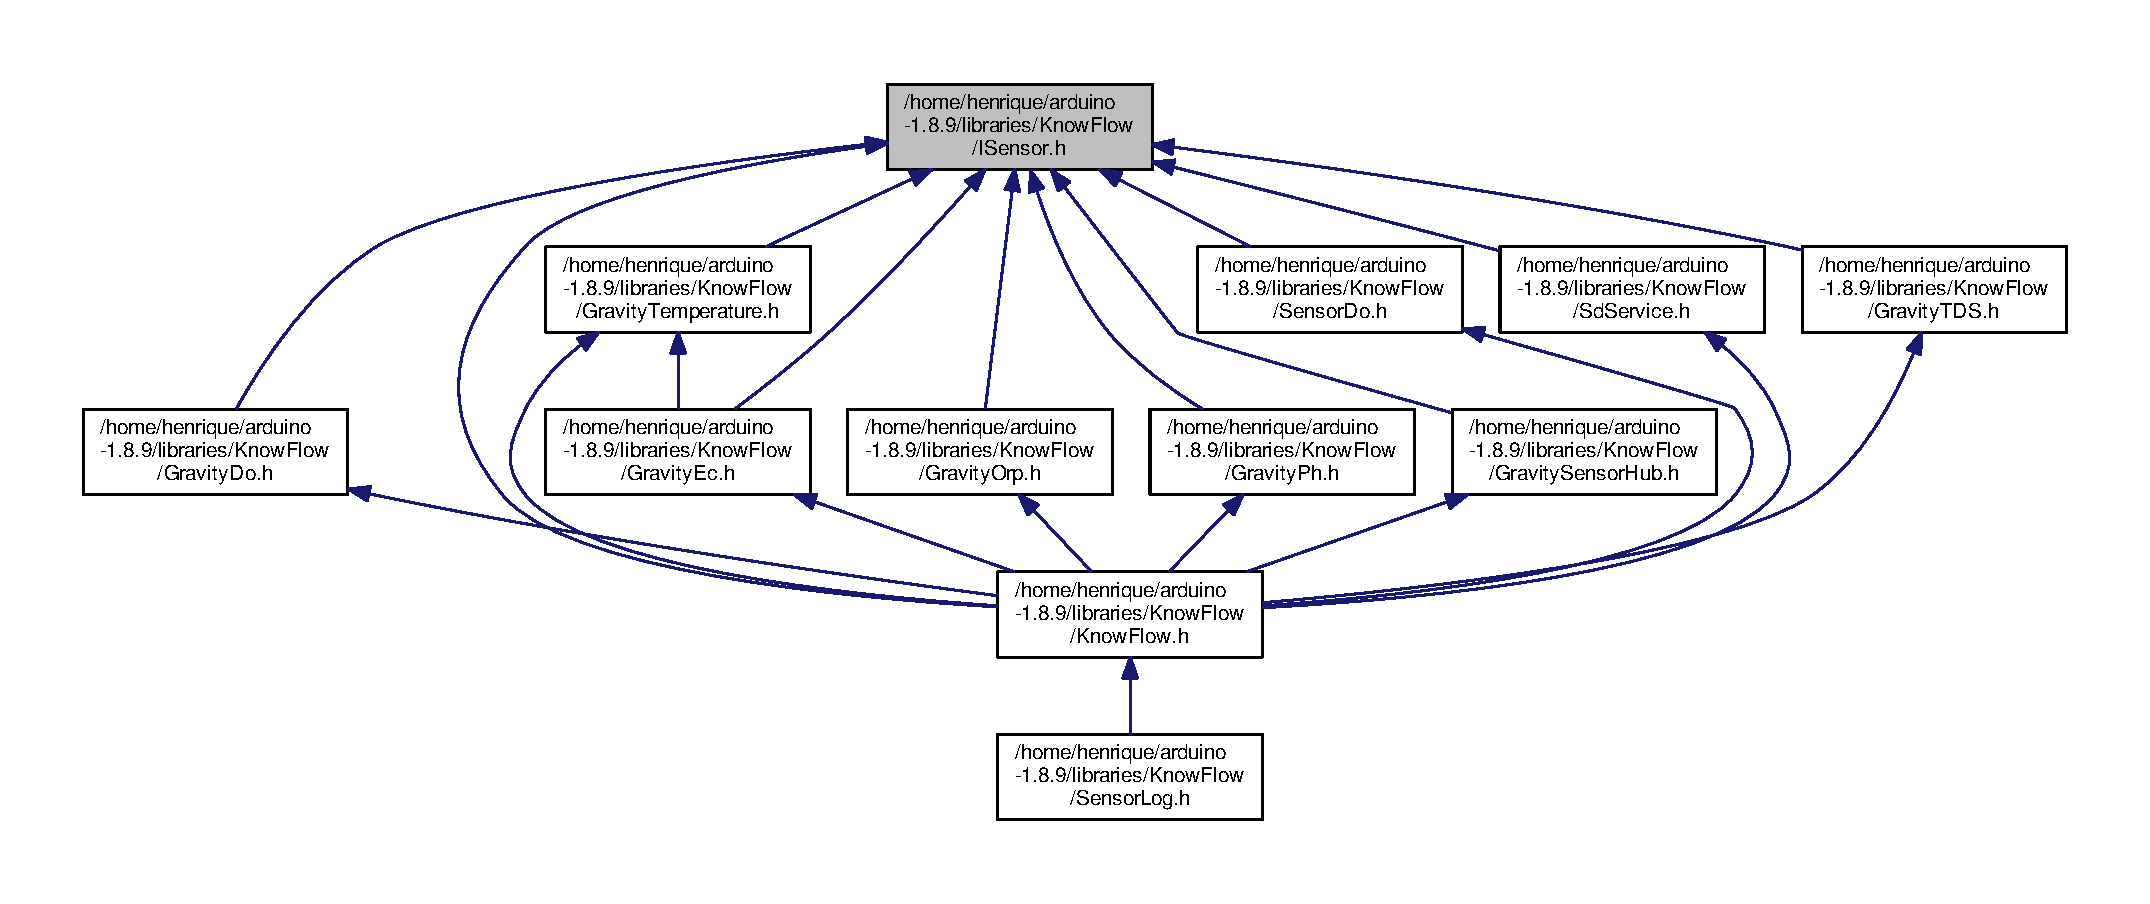
\includegraphics[width=350pt]{_i_sensor_8h__dep__incl}
\end{center}
\end{figure}
\subsection*{Classes}
\begin{DoxyCompactItemize}
\item 
class \hyperlink{class_i_sensor}{I\+Sensor}
\end{DoxyCompactItemize}


\subsection{Detailed Description}
This class represents a generic sensor. 

\begin{DoxyAuthor}{Author}
Jason(\href{mailto:jason.ling@dfrobot.com}{\tt jason.\+ling@dfrobot.\+com}) 
\end{DoxyAuthor}
\begin{DoxyDate}{Date}
2017-\/04-\/06 
\end{DoxyDate}

%--- End generated contents ---

% Index
\backmatter
\newpage
\phantomsection
\clearemptydoublepage
\addcontentsline{toc}{chapter}{Index}
\printindex

\end{document}
